\documentclass[12pt,a4paper,%
%draft%
]{scrreprt}
% prevent warning \float@addtolists detected
\usepackage{scrhack} 

% Textkodierung Deutsch
\usepackage[ngerman]{babel}
\usepackage[T1]{fontenc}
\usepackage[utf8]{inputenc}
\usepackage{lmodern}
\usepackage{xspace}
\usepackage{microtype}

% Basisinfos
\title{Modellbasierte Testautomatisierung eines verteilen, adaptiven Load-Balancing-Systems}
\author{Gerald Siegert}
\date{\today}
%Variablen welche innerhalb der gesamten Arbeit zur Verfügung stehen sollen
\newcommand{\titleDocument}{Masterarbeit}
\newcommand{\subjectDocument}{im Studiengang Informatik}
\newcommand{\zB}{z.\,B. }
\newcommand{\uA}{u.\,A. }
\newcommand{\sS}{S\# }
\newcommand{\cS}{C\# }
\newcommand{\uU}{u. U.}
\newcommand{\isse}{Institute for Software \& Systems Engineering}

%hier müssen alle Wörter rein, welche Latex von sich auch nicht korrekt trennt bzw. bei denen man die genaue Trennung vorgeben möchte
\hyphenation
{
    Film-pro-du-zen-ten
    Lux-em-burg
    Soft-ware-bau-steins
    zeit-in-ten-siv
}
\renewcommand{\texttt}[1]{%
    \begingroup
    \ttfamily
    \begingroup\lccode`~=`/\lowercase{\endgroup\def~}{/\discretionary{}{}{}}%
    \begingroup\lccode`~=`[\lowercase{\endgroup\def~}{[\discretionary{}{}{}}%
    \begingroup\lccode`~=`.\lowercase{\endgroup\def~}{.\discretionary{}{}{}}%
    \catcode`/=\active\catcode`[=\active\catcode`.=\active
    \scantokens{#1\noexpand}%
    \endgroup
}

% Seitenränder
\usepackage{geometry}
\geometry{left=35mm,right=20mm,top=25mm,bottom=20mm}

% Kopf/Fußzeilen
\usepackage[headsepline]{scrlayer-scrpage}
\clearscrheadfoot
\pagestyle{scrheadings}

\ihead{\headmark}
\automark{chapter}
\ohead{\pagemark}

\renewcommand*{\headfont}{\normalfont}
\setlength{\headheight}{1.5\baselineskip}
\renewcommand*{\chapterpagestyle}{scrheadings}

\newpairofpagestyles[scrheadings]{lists}{%
    \ihead{Verzeichnisse}%
    }

% Grafiken
\usepackage{graphicx}
\usepackage{wrapfig}
\usepackage[format=plain]{caption}
\setkeys{Gin}{width=0.8\columnwidth} % default width
 
% Tabellen
\usepackage{multirow}

% Textfarben
\usepackage{xcolor}

% Abkürzungen
\usepackage[nohyperlinks,printonlyused]{acronym}

% Zeilenabstand
\usepackage[onehalfspacing]{setspace}
\usepackage{enumitem}
\setlist[itemize]{noitemsep} % noitemsep bei listen
\renewcommand*{\chapterheadstartvskip}{\vspace*{.5\baselineskip}}% Abstand vor Kapiteltitel

% Literatur
\usepackage[style=numeric-comp,natbib=true,maxitems=1,backend=biber,sorting=none]{biblatex}
\usepackage{csquotes}
\addbibresource{./literatur.bib}
\addbibresource{./web.bib}
\addbibresource{./abbildungen.bib}
% Zeilenumbrüche bei URLs
\setcounter{biburllcpenalty}{7000}
\setcounter{biburlucpenalty}{8000}

% Listings
\usepackage{listings}
\makeatletter
\definecolor{bluekeywords}{rgb}{0.13,0.13,1}
\definecolor{greencomments}{rgb}{0,0.5,0}
\definecolor{redstrings}{rgb}{0.9,0,0}
\definecolor{typeidentifier}{RGB}{38, 121,	153}
\lstdefinestyle{base}{
    basicstyle=\footnotesize\ttfamily,
    frame=single,
    numbers=left,
    numberstyle=\tiny,
    numbersep=7pt,
    breaklines=true,
    tabsize=3,
    captionpos=b,
    extendedchars=true,
    showstringspaces=false,
}
\lstdefinestyle{cs}{
    language=[sharp]c,
    style=base,
    escapeinside={(*@}{@*)},
    morekeywords={get,set,var,nameof},
    moredelim=[is][\color{typeidentifier}]{|}{|},
    commentstyle=\color{greencomments},
    keywordstyle=\color{bluekeywords}\bfseries,
    stringstyle=\color{redstrings},
}
\lstdefinestyle{plain}{
    language={},
    style=base,
    tabsize=4,
    captionpos=t,
}
% Json Listings
\newcommand\JSONnumbervaluestyle{\color{blue}}
\newcommand\JSONstringvaluestyle{\color{red}}
% switch used as state variable
\newif\ifcolonfoundonthisline
\lstdefinestyle{json}
{
    style=base,
    captionpos=t,
    showstringspaces    = false,
    keywords            = {false,true},
    alsoletter          = 0123456789.,
    morestring          = [s]{"}{"},
    stringstyle         = \ifcolonfoundonthisline\JSONstringvaluestyle\fi,
    MoreSelectCharTable =%
    \lst@DefSaveDef{`:}\colon@json{\processColon@json},
    basicstyle          = \ttfamily,
    keywordstyle        = \ttfamily\bfseries,
}
% flip the switch if a colon is found in Pmode
\newcommand\processColon@json{%
    \colon@json%
    \ifnum\lst@mode=\lst@Pmode%
    \global\colonfoundonthislinetrue%
    \fi
}
\lst@AddToHook{Output}{%
    \ifcolonfoundonthisline%
    \ifnum\lst@mode=\lst@Pmode%
    \def\lst@thestyle{\JSONnumbervaluestyle}%
    \fi
    \fi
    %override by keyword style if a keyword is detected!
    \lsthk@DetectKeywords% 
}
% reset the switch at the end of line
\lst@AddToHook{EOL}%
{\global\colonfoundonthislinefalse}
%%%%%%%%%% end listings

\makeatletter

% Default centering floatboxes
\g@addto@macro\@floatboxreset\centering

% Verzeichnisse
\renewcommand\listoffigures{%
    \addsec{\listfigurename}%
    \@mkboth{\MakeUppercase\listfigurename}%
    {\listfigurename}%
    \@starttoc{lof}%
}
\renewcommand\listoftables{%
    \addsec{\listtablename}%
    \@mkboth{\MakeUppercase\listtablename}%
    {\listtablename}%
    \@starttoc{lot}%
}
\renewcommand\lstlistoflistings{%
    \addsec{\lstlistlistingname}%
    \@mkboth{\MakeUppercase\lstlistlistingname}%
    {\lstlistlistingname}%
    \@starttoc{lol}%
}

\makeatother

% Hurenkinder, Schusterjungen
\clubpenalty = 10000
\widowpenalty = 10000
\displaywidowpenalty = 10000 

% Referenzen
\PassOptionsToPackage{hyphens}{url}\usepackage{hyperref}

\usepackage{todonotes}
\presetkeys{todonotes}{inline}{}

\begin{document}
    % Titelseite
    \setcounter{page}{-100}
    \begin{titlepage}
        \begin{doublespace}
            \thispagestyle{empty}

\begin{figure}[t]
\centering
% \includegraphics[width=0.6\textwidth]{abb/logo1}
~~~~~~~~~~
% \includegraphics[width=0.3\textwidth]{abb/logo2}
\end{figure}


\begin{verbatim}


\end{verbatim}

\begin{center}
\Large{Universität Augsburg}\\
\end{center}


\begin{center}
\Large{Fakultät für Angewandte Informatik}
\end{center}
\begin{verbatim}




\end{verbatim}
\begin{center}
\doublespacing
\textbf{\LARGE{Masterarbeit}}\\
\singlespacing
\begin{verbatim}

\end{verbatim}
\textbf{{~im Studiengang Informatik~}}
\end{center}
\begin{verbatim}

\end{verbatim}
\begin{center}

\end{center}
\begin{verbatim}

\end{verbatim}
\begin{center}
\textbf{zur Erlangung des akademischen Grades \\\ \\ Master of Science}
\end{center}
\begin{verbatim}






\end{verbatim}
\begin{flushleft}
\begin{tabular}{llll}
\textbf{Thema:} & & <Thema der Arbeit> & \\
& & \\
\textbf{Autor:} & & Gerald Siegert & \\
& & MatNr. 1450117 & \\
& & \\
\textbf{Version vom:} & & \today &\\
& & \\
\textbf{Betreuer:} & & M.Sc. Benedikt Eberhardinger &\\
\textbf{1. Prüfer:} & & Prof. Dr. X &\\
\textbf{2. Prüfer:} & & Prof. Dr. Y &\\
\end{tabular}
\end{flushleft}
        \end{doublespace}
    \end{titlepage}
    
    % Abstract
    \pagenumbering{Roman}
    \begin{abstract}
    Durch eine Automatisierung von Tests lassen sich im Bereich der Softwareentwicklung hohe Kosten einsparen.
    Daher wurden zahlreiche Test"=Frameworks und Möglichkeiten zum Testen von Systemen und ihrer Software entwickelt.
    Ein solches Framework ist \acrshort{ss} (\acrlong{ss}), mit dem mithilfe eines modellbasierten Ansatzes Systeme getestet werden können.
    Mithilfe des \acrshort{ss}"=Frameworks soll nun ein Testsystem entwickelt werden, um hiermit automatisiert ein verteiltes, adaptives Load"=Balancing"=System zu testen.
    Hierfür wurde Apache Hadoop ausgewählt, welches mit einer selbstadaptiven Komponente ergänzt wird.
    Diese selbstadaptive Komponente verändert dynamisch und basierend auf den derzeit auf dem Hadoop"=Cluster ausgeführten Anwendungen einige der sonst statischen Einstellungen von Hadoop, womit die verfügbaren Ressourcen des Clusters optimaler genutzt werden können.
    
    Um Hadoop testen zu können, wurde zunächst mithilfe von \acrshort{ss} ein Modell entwickelt, welches die wesentlichen Komponenten des \acrshort{YARN}"=Frameworks von Hadoop abbildet.
    Dieses Modell wurde wiederum mithilfe eines hierfür entwickelten Treibers mit einem realen Hadoop"=Cluster verbunden.
    Dadurch wurde es ermöglicht, durch die Testausführung mit \acrshort{ss} unterschiedliche Anwendungen auf dem realen Cluster auszuführen und die Daten der Anwendungen und des Clusters im Modell zu nutzen.
    Um zu testen, ob sich das entwickelte Testsystem zur Testautomatisierung eines verteilten, adaptiven Load"=Balancing"=Systems eignet, wurde hierfür eine Fallstudie durchgeführt.
    
    In dieser Masterarbeit werden der Aufbau und Ablauf der durchgeführten Fallstudie, sowie die Entwicklung und Implementierung des hierfür genutzten Testsystems erläutert.
    Es wird gezeigt, welche Besonderheiten bei der Durchführung und Auswertung der Fallstudie aufgetreten sind, und inwiefern sich das entwickelte, modellbasierte Testsystem zur Testautomatisierung eines verteilten, adaptiven Load"=Balancing"=Systems eignet.
\end{abstract}

\clearpage
\begin{otherlanguage}{english}
\begin{abstract}
    By automating tests, high costs can be saved in software development.
    Therefore, numerous test frameworks and ways to test systems and their software have been developed.
    One such framework is \acrshort{ss} (\acrlong{ss}), which uses a model-based approach to test systems.
    By using the \acrshort{ss} framework, a test system will be developed to automatically test a distributed, adaptive load-balancing system.
    For this, Apache Hadoop was chosen, which is equipped with an adaptive resource manager.
    The manager detect the current usage of the cluster and modify some of Hadoop's otherwise static settings to make a better use of the available resources.
    
    To test hadoop, a \acrshort{ss} model was developed, which contains the essential componentens of the Hadoop \acrshort{YARN} framework.
    To connect the model to a real Hadoop cluster a driver was developed for this purpose.
    This allows \acrshort{ss} to run different applications on the real cluster and detect the state of the running applications and the cluster.
    To determine the developed test system is suitable for the test automation of a distributed, adaptive load-balancing system, a case study was performed.
    
    This master thesis explains the structure and processes of the case study, as well as the development and implementation of the test system used for this purpose.
    It shows the won experiences by performing the case study and shows how the developed, model-based test system is suitable for test automation of a distributed, adaptive load-balancing system.
\end{abstract}
\end{otherlanguage}


    
    % Verzeichnisse
    \pagestyle{lists}
    \newpage
    \begin{singlespace}
        \tableofcontents
        \addchap{Verzeichnisse}

%\renewcommand{\listfigurename}{Abbildungen}
\listoffigures

%\renewcommand{\lstlistlistingname}{Listings}
\lstlistoflistings

%\renewcommand{\listtablename}{Tabellen}
\listoftables

%\section*{Abkürzungen}\addcontentsline{toc}{section}{Abkürzungen}
\addsec{Abkürzungsverzeichnis}%\addcontentsline{toc}{section}{Abkürzungsverzeichnis}
\begin{acronym}[AppMstr]
    \acro{AM}{ApplicationManager}
    \acro{AppMstr}{ApplicationMaster}
    \acro{DCCA}{Deductive Cause-Consequence Analysis}
    \acro{MARP}{\texttt{maximum-am-resource-percent}}
    \acro{MC}{Model Checking}
    \acro{MCr}[MC]{Model Checker}
    \acro{NM}{NodeManager}
    \acro{RM}{ResourceManager}
    \acro{TLS}{Timeline-Server}
\end{acronym}
    \end{singlespace}
    
    % Inhalt
    \pagestyle{scrheadings}
    \newpage
    \pagenumbering{arabic}
    
    \chapter{Einleitung}
\label{ch:intro}

Im Bereich der Softwaretests wird heutzutage sehr viel mit automatisierten Testverfahren gearbeitet.
Dies ist insofern logisch, als dass diese Testautomatisierung einerseits Aufwand und damit andererseits direkt Kosten einer Software einspart.
Daher gibt es vor allem im Bereich der Komponententests zahlreiche Frameworks, mit denen Tests einfach und automatisiert erstellt bzw. ausgeführt werden können.
Ein Beispiel für ein solches Testframework wäre das \emph{xUnit}"=Framework, zu dem \uA JUnit\footnote{\url{https://junit.org}} für Java und NUnit\footnote{\url{https://nunit.org/}} für .NET zählen.
Dabei werden zunächst einzelne Testfälle erstellt und können im Anschluss mit der jeweils aktuellen Codebasis jederzeit ausgeführt werden.
Automatisierte Tests können auch dazu genutzt werden, um einen einzelnen Test mit verschiedenen Eingaben durchzuführen.
Dadurch können verschiedene Eingabeklassen (wie negative oder positive Ganzzahlen) mit sehr geringem Aufwand in einem Test genutzt werden und somit verschiedene Testfälle direkt ausgeführt werden, wodurch eine massive Kosteneinsparung einhergeht \cite{Polo2013}.

Es gibt aber nicht nur Frameworks für Komponententests, sondern auch für modellbasierte Testverfahren wie \zB dem \ac{MC}.
Beim \ac{MC} wird ein Modell mithilfe eines entsprechenden Frameworks automatisiert auf seine Spezifikation getestet und geprüft, unter welchen Umständen diese verletzt wird \cite{Grumberg1999,Habermaier2015}.

In dieser Masterarbeit soll daher nun ein verteiltes, adaptives Load"=Balancing"=System getestet werden.
Hauptziel ist es, zu ermitteln, wie ein modellbasierter Testansatz auf ein komplexes Beispiel übertragen werden kann.
Dafür wird zunächst ein reales System als vereinfachtes Modell nachgebildet und anschließend mithilfe eines \ac{MC} getestet.
Es soll dabei auch ermittelt werden, wie ein reales System in das Modell eingebunden werden kann und wie bei Problemen mit asynchronen Prozessen innerhalb des verteilten Systems umgegangen werden muss.

\todo{vielleicht Testing MapReduce-Based Systems einbringen?}

    %\chapter{Relevante Methodiken}\label{chap:methodiken}

\section{Model Checking}\label{sec:modelchecking}

\ac{MC} ist eine Möglichkeit, um Systeme zu testen und zu verifizieren. Dazu werden vom \ac{MCr} alle möglichen Systemzustände in einem \emph{brute-force}-ähnlichem Vorgehen getestet und somit alle möglichen Szenarien getestet. Die Anzahl der Zustände kann sehr schnell $ 10^{120} $ oder mehr betragen \cite{Grumberg1999,Baier2008}.

\begin{figure}
	\includegraphics{./images/mcSchema.pdf}
	\caption[Schematischer Aufbau beim MC]{Schematischer Aufbau beim MC, nach \cite{Baier2008}}
	\label{fig:mcSchema}
\end{figure}

Ein \ac{MCr} nutzt, wie der Name schon sagt, ein Modell des Systems, um das System zu testen. Wie bei jeder anderen modellbasierten Technik ist daher die Qualität des \ac{MC} nur so gut wie das darauf zugrunde liegende Modell. Ein Modell kann auch als endlicher Automat angesehen werden, da ein Modell ebenfalls eine endliche Anzahl an möglichen Zuständen und dazugehörige Übergänge besitzt. Für jede Eigenschaft eines Zustandes muss zudem mithilfe einer sog. \emph{temporalen Logik}, also mathematisch bzw. formal, festgelegt werden, was gültige Werte dieser Eigenschaft sind. Die dazu benötigten Informationen werden aus den Anforderungen des Systems ermittelt und dem \ac{MCr} übergeben. So können später verschiedene Eigenschaften des gesamten Systems (\zB die formale Korrektheit, die Ausführbarkeit ohne Deadlocks oder die Einhaltung von Sicherheitsvorgaben) geprüft werden.

Zur Ausführung wird das gesamte Modell zunächst initialisiert und dann automatisch und systematisch vom \ac{MCr} auf Fehler und ungültige Zustände geprüft. In der Regel ist aber auch eine Ausführung als reine Simulation des Systems möglich, ohne explizit nach Fehlern zu suchen.

Wenn alle Zustände und deren Eigenschaften die Anforderungen erfüllen, erfüllt auch das Modell die Spezifikation. Wenn ein Zustand bzw. Eigenschaft die Anforderungen nicht erfüllt, prüft der \ac{MCr} anhand eines Gegenbeispiels den Ausführungspfad zum Fehler. Dadurch kann ermittelt werden, wo die Fehlerursache liegt. Einige der wesentlichen Fehlertypen und Ursachen sind:

\begin{description}
	\item[Modelling Error] Der Fehler liegt im Modell, welches korrigiert werden muss.
	\item[Design Error] Der Fehler liegt in den formellen oder informellen Anforderungen, dadurch muss das Modell und/oder die temporale Logik korrigiert werden.
	\item[Property Error] Der Fehler ist wirklich ein Fehler im System, welcher gefunden werden soll.
\end{description}

Möglich ist aber auch, dass die Ressourcen nicht ausreichen, um alle Zustände zu prüfen. In so einem Fall gibt es mehrere Möglichkeiten, damit umzugehen, \zB können Heuristiken oder Abstraktionen vom Modell genutzt werden \cite{Baier2008,Eberhardinger2016}.

\ac{MC} besitzt durch seine Charakteristik einige Vorteile, \uA \cite{Baier2008}:
\begin{itemize}
	\item \ac{MC} ist universell nutzbar, \zB für Software, Hardware oder eingebettete Systeme
	\item Partielle Verifikation ist möglich ohne das gesamte System testen zu müssen
	\item Vollständig automatisierbar und benötigt kaum Benutzerinteraktion oder hohe Expertise
\end{itemize}

Natürlich gibt es aber auch einige Nachteile, \uA \cite{Baier2008}:
\begin{itemize}
	\item Mit \ac{MC} wird nur ein Systemmodell und nicht das eigentliche System getestet, was weitere Fehler nicht ausschließt
	\item Hauptsächlich für steuerungsbasierte Anwendungen und nicht für datenbasierte Anwendungen geeignet
	\item Anzahl der möglichen Zustände kann zu hoch sein, um alle zu testen
\end{itemize}

Es gibt zahlreiche \ac{MC}-Frameworks, die bereits erwähnten \emph{LTSmin} und \emph{\sS} sind nur zwei davon.

\section{\acl{ss}}
\label{sec:ssharp}

\todo{Testen unter SS allgemein genauer erklären und an neue Abschnitte anpassen}
\textbf{\acf{ss}} ist ein am \isse der Universität Augsburg entwickeltes Framework zum Testen und Verifizieren von Systemen und Modellen.
Da es in \cS entwickelt wurde und \cS auch zum Entwickeln von Modellen und dazugehörigen Testszenarien genutzt wird, können zahlreiche Features des .NET"=Frameworks bzw. der Sprache \cS im Speziellen genutzt werden.
\ac{ss} vereint dabei die Simulation, die Visualisierung, modellbasierte Tests sowie die Verifizierung der Modelle durch einen \ac{MCr} \cite{Habermaier2015,Habermaier2016}.
Dadurch können alle Schritte einer vollständigen Analyse inkl. Modellierung direkt im Visual Studio ausgeführt werden und somit auch alle Features der IDE und .NET, wie \zB die Debugging"=Werkzeuge, genutzt werden.
Um entsprechende Analysen zu gewährleisten, hat das Framework jedoch auch einige Einschränkungen, wodurch \zB Schleifen und Rekursionen nur eingeschränkt bzw. nicht möglich sind.
Eine der größten Einschränkungen ist allerdings, dass während der Laufzeit keine neuen Objektinstanzen innerhalb des zu testenden Modells erzeugt werden können, sodass alle benötigten Instanzen bereits während der Initialisierung des Modells erzeugt werden müssen \cite{Habermaier2015}.

\subsection{Aufbau eines Modells}
\label{subsec:ssharpModel}

\todo{Hier Oracle, Modell selbst und so rein}

Um nun ein System testen zu können, muss dieses zunächst mithilfe von \cS-Klassen und -Instanzen modelliert werden.
Die dafür verwendeten Modelle sind meist stark vereinfacht und bilden nur die wesentlichen Aspekte der realen Systeme ab.
Für einen korrekten Test ist es jedoch wichtig, dass das Modell des Systems vergleichbar mit dem echten System ist.

Folgendes Beispiel zeigt den typischen, grundlegenden Aufbau einer \ac{ss}-Komponente:

\begin{lstlisting}[label=lst:ssExample,style=cs,
caption={Grundlegender Aufbau einer \acs{ss}-Komponente.}]
public class MyCOmponent : Component
{
  // fault definition, also possible: n§§ew PermanentFault()
  public readonly Fault MyFault = new TransientFault();
  
  // interaction logic (Fields, Properties, Methods...)
  
  // fault effect
  [FaultEffect(Fault = nameof(MyFault))]
  internal class MyFaultEffect : MyCOmponent
  {
    // fault effect logic
  }
}
\end{lstlisting}

Jede Komponente des Modells muss von \texttt{Component} erben, um als \ac{ss}-Komponente definiert zu sein.
Jede Komponente kann nun temporäre (\texttt{TransientFault}) oder dauerhafte (\texttt{PermanentFault}) Komponentenfehler enthalten, welche zunächst innerhalb der Komponente als Felder definiert werden. 
Der Effekt eines Komponentenfehlers wird anschließend in der entsprechenden Effekt"=Klasse definiert, welche von der Hauptklasse (hier \texttt{YarnNode}) erbt und mithilfe des Attributs \texttt{FaultEffectAttribute} dem dazugehörigen Komponentenfehler zugeordnet wird \cite{Habermaier2016}.

\subsection{Ausführung eines Modells mit \acs{ss}}
\label{subsec:ssharpExecution}

Um die Modelle zu testen, kommen in \ac{ss} verschiedene Werkzeuge zum Einsatz.
Eines davon ist eine reine Simulation, bei der das Framework nur einen Ausführungspfad ausführt und dabei keine Komponentenfehler aktiviert bzw. die Aktivierung \textit{manuell} gesteuert werden kann.
Ein weiterer Nutzen liegt in der Möglichkeit, im ausgeführten Ausführungspfad zeitliche Abläufe zu berücksichtigen, da hier das Modell Schritt für Schritt ausgeführt wird.
Hierbei wird für jede im Modell genutzte Komponente pro Schritt einmal die jeweilige Methode \texttt{Update()} aufgerufen, in der die jeweiligen Komponenten ihre Aktivitäten durchführen \cite{Habermaier2016}.

Ein anderes wichtiges Werkzeug von \ac{ss} ist die \ac{DCCA}, welche eine vollautomatische und \ac{MC}-basierte Sicherheitsanalyse ermöglicht.
Dabei wird selbstständig die Menge der aktivierten Komponentenfehler ermittelt, mit denen das Gesamtsystem nicht mehr rekonfiguriert werden kann und somit ausfällt.
Je nach Konfiguration können dazu auch Heuristiken genutzt werden, welche die Analyse beschleunigen und genauer machen können \cite{Eberhardinger2016}.
Dabei werden die verschiedenen aktivierten Komponentenfehler während der Analyse in tolerierbare und nicht-tolerierbare Fehler unterschieden.
Tolerierbare Komponentenfehler werden dazu genutzt, die Grenzen der Selbstkonfiguration des Systems zu ermitteln.
Dabei wird für jeden Systemzustand nach einer Rekonfiguration durch die \ac{DCCA} eine neue Fehlermenge ermittelt, mit der das System gerade noch lauffähig ist.
Das Auftreten eines tolerierbaren Komponentenfehler ist also gleichbedeutend mit einem einfachen Fehler im System, welcher die gesamte Funktionsweise des Systems nicht massiv einschränkt und eine Rekonfiguration noch ermöglicht.
Sobald jedoch ein Fehler auftritt, durch den eine Rekonfiguration des Systems nicht mehr möglich ist, wurde ein nicht-tolerierbarer Fehler gefunden, durch den das System nicht mehr funktionsfähig ist \cite{Habermaier2015}.

Das dritte Werkzeug zur Ausführung von Modellen in \ac{ss} ist der \ac{MCr} selbst.
Hierbei kann der in \ac{ss} bereits enthaltene, oder alternativ \emph{LTSmin}\footnote{\url{http://ltsmin.utwente.nl/}} genutzt werden \cite{SSWikiModelChecking}.
Beim \ac{MC} werden in einem \emph{brute-force}-ähnlichem Verfahren alle möglichen Zustände und Ausführungspfade in einem Modell mit einer endlichen Anzahl an Zuständen getestet.
Dadurch wird es ermöglicht, verschiedene Eigenschaften eines System zu testen und Fehler (\zB Deadlocks) zu erkennen \cite{Grumberg1999}.

    \chapter{Fallstudie}\label{sec:fallstudie}

\input{./fallstudie/ablauf}

\section{Apache Hadoop}\label{sec:hadoop}

\textbf{Apache Hadoop} ist ein Open-Source-Software-Projekt, mit dessen Hilfe ermöglicht wird, Programme zur Datenverarbeitung mit großen Ressourcenbedarf auf verteilten System auszuführen. Hadoop wird von der \emph{Apache Foundation} entwickelt und bietet verschiedene Komponenten an, welche vollständig skalierbar sind, von einer einfachen Installation auf einem PC bis hin zu einer Installation über mehrere Server in einem Serverzentrum. Hadoop besteht hauptsächlich aus folgenden Kernmodulen \cite{HadoopHomePage}:

\begin{description}
	\item[Hadoop Common] Gemeinsam genutzte Kernkomponenten
	\item[Hadoop YARN] Framework zur Verteilung und Ausführung von Anwendungen und das dazugehörige Ressourcen-Management
	\item[Hadoop Distributed File System] Kurz HDFS, Verteiltes Dateisystem
	\item[Hadoop MapReduce] YARN-Basiertes System zum Verarbeiten von großen Datenmengen
\end{description}

Hadoop ermöglicht es dadurch, sehr einfach mit Anwendungen umzugehen, welche große Datenmengen verarbeiten. Da es für Hadoop nicht relevant ist, auf wie vielen Servern es läuft, kann es beliebig skaliert werden, wodurch entsprechend viele Ressourcen zur Bearbeitung und Speicherung von großen Datenmengen zur Verfügung stehen können.

\begin{figure}
	\centering
	\includegraphics[width=\columnwidth]{./images/yarn_architecture.png}
	\caption[Architektur von YARN]{Architektur von YARN (entnommen aus \cite{HadoopYarnArch271})}
	\label{fig:yarnarch}
\end{figure}

Die Kernidee der Architektur von \textbf{YARN} ist die Trennung vom Ressourcenmanagement und Scheduling. Dazu besitzt der Master bzw. \emph{Controller} den \ac{RM}, welcher für das gesamte System zuständig ist und die Anwendungen im System verteilt und überwacht und somit auch als \emph{Load-Balancer} agiert. Er besteht aus zwei Kernkomponenten, dem \ac{AM} und dem \emph{Scheduler}. Der \ac{AM} ist für die Annahme und Ausführung von einzelnen Anwendungen zuständig, denen der Scheduler die dafür notwendigen Ressourcen im Cluster zuteilt.

Jeder Slave-\emph{Node} im Hadoop-Cluster besitzt einen \ac{NM}, welcher für die Überwachung der Ressourcen des Nodes und der darauf ausgeführten Anwendungs-Container zuständig ist und diese dem \ac{RM} mitteilt.

Jede YARN-Anwendung bzw. Job besteht aus einem oder mehreren Ausführungsversuchen, genannt \emph{Attempts}, denen wiederum mehrere \emph{Container} zugeordnet sind. Container können auf einem beliebigen Node ausgeführt werden und repräsentieren die Ausführung eines Tasks der Anwendung. Ein besonderer Container bildet dabei der \ac{AppMstr}, welcher innerhalb seines Attempts für das anwendungsbezogene Monitoring und die Kommunikation mit dem \ac{RM} und \ac{NM} zuständig ist und die dazu notwendigen Informationen bereit stellt \cite{HadoopYarnArch271}.

Hadoop enthält zudem einen sog. \ac{TLS}. Er ist speziell dafür entwickelt, die Metadaten und Logs der YARN-Anwendungen zu speichern und jederzeit, also auch als Anwendungshistorie, auszugeben \cite{HadoopYarnTlServer271}.

\begin{figure}
    \centering
    \includegraphics[width=.8\columnwidth]{./images/hdfsarchitecture.png}
    \caption[Architektur des HDFS]{Architektur des HDFS (entnommen aus \cite{HadoopHdfsDesc271})}
    \label{fig:hdfsarch}
\end{figure}

Das \textbf{HDFS} basiert auf der gleichen Architektur wie YARN und besitzt ebenfalls einen Master und mehrere Slaves, welches in der Regel die gleichen Nodes sind wie bei YARN sind. Der \emph{NameNode} ist als Master für die Verwaltung des Dateisystems zuständig und reguliert den Zugriff auf die darauf gespeicherten Daten. Die Daten selbst werden in mehrere Blöcke aufgeteilt auf den \emph{DataNodes} gespeichert. Um den Zugriff auf die Daten im Falle eines Node-Ausfalls zu gewährleisten, wird jeder Block auf anderen Nodes repliziert. Dateioperationen (wie Öffnen oder Schließen) werden direkt auf den DataNodes ausgeführt, sie sind darüber hinaus auch dafür verantwortlich, dass Clients die Daten lesen oder beschreiben können \cite{HadoopHdfsDesc271}.

\textbf{MapReduce} bietet analog zu YARN die Möglichkeit, Anwendungen mit einem großen Ressourcenbedarf, welche große Datenmengen verarbeiten, auf einem gesamten Cluster auszuführen. Dazu werden bei einem MapReduce-Job die Eingabedaten aufgeteilt, anschließend von den sog. \emph{Map Tasks} verarbeitet und deren Ausgaben von den sog. \emph{Reduce Tasks} geordnet. Für die Ein- und Ausgabe der Daten wird in der Regel das HDFS, für die Ausführung der einzelnen Tasks YARN genutzt \cite{HadoopMapRedTutorial271}. MapReduce kann auch als Vorgänger von YARN angesehen werden, da YARN auch als \emph{MapReduce Next Gen} bzw. \emph{MRv2} bezeichnet wird und aufgrund der API-Kompatibilität von YARN jede MapReduce-Anwendung in der Regel auch auf YARN ausgeführt werden kann \cite{HadoopYarnArch271,HadoopYarnOverview271}.


\section{Adaptive Komponente in Hadoop}\label{sec:inriaSetting}

Ein normales Hadoop besitzt von Haus aus keine adaptive Komponente, sondern rein statische Einstellungen. Um damit Hadoop zu optimieren, müssen die Einstellungen immer manuell auf den jeweils benötigten Anwendungstyp angepasst werden. Dazu gibt es auch bereits verschiedene Scheduler, den \emph{Fair Scheduler}, welcher alle Anwendungen ausführt und ihnen gleich viele Ressourcen zuteilt, und den \emph{Capacity Scheduler}. Letzterer sorgt dafür, dass nur eine bestimmte Anzahl an Anwendungen pro Benutzter gleichzeitig ausgeführt wird und teilt ihnen so viele Ressourcen zu, wie benötigt werden bzw. der Benutzter nutzen darf. Entwickelt wurde der Capacity Scheduler vor allem für Cluster, die von mehreren Organisationen gemeinsam verwendet werden und sicherstellen soll, dass jede Organisation eine Mindestmenge an Ressourcen zur Verfügung hat \cite{HadoopCapScheduler271}.

Je nach Bedarf besitzt der Capacity Scheduler entsprechende Einstellungen, um \zB den verfügbaren Speicher pro Container festzulegen. Eine weitere Einstellung des Schedulers ist \texttt{maximum-am-resource-percent}, auch MARP genannt, der angibt, wie viele Prozent der gesamten Ressourcen durch \ac{AppMstr} genutzt werden dürfen \cite{HadoopCapScheduler271}. Damit bewirkt diese Einstellung indirekt auch die maximale Anzahl an Anwendungen, die gleichzeitig ausgeführt werden dürfen. Da der MARP-Wert jedoch nicht während der Laufzeit dynamisch angepasst werden kann, haben \citeauthor{zhang2016} in \cite{zhang2016} einen Ansatz zur dynamischen Anpassung des MARP-Wertes zur Laufzeit von Hadoop vorgestellt. Dadurch wird der MARP-Wert abhängig von den ausgeführten Anwendungen adaptiv zur Laufzeit angepasst, sodass immer möglichst viele Anwendungen gleichzeitig ausgeführt werden können. Gemäß \citeauthor{zhang2016} werden dadurch Anwendungen im Schnitt um bis zu 40 \% schneller ausgeführt.

\begin{figure}
    \centering
    \includegraphics[width=.8\columnwidth]{./images/marpValue.pdf}
    \caption[LoJP und LoJT in Hadoop]{LoJP und LoJT in Hadoop \cite{zhang2016}}
    \label{fig:marpValue}
\end{figure}

Der Hintergrund dieser \emph{Selfbalancing-Komponente} ist der, dass durch den MARP-Wert der für die Anwendungen verfügbare Speicher in zwei Teile aufgeteilt wird. Im einen Teil befinden sich alle derzeit ausgeführten \ac{AppMstr}, im anderen Teil die von den Anwendungen benötigten weiteren Container. Wie groß der Teil für die \ac{AppMstr} ist, wird nun durch den MARP-Wert bestimmt. Ist der MARP-Wert zu klein, können nur wenige \ac{AppMstr} (und damit Anwendungen) gleichzeitig ausgeführt werden (\emph{Loss of Jobs Parallelism}, LoJP). Ist der MARP-Wert jedoch zu groß, können für die ausgeführten Anwendungen nur wenige Container bereitgestellt werden, wodurch sich die Ausführung für eine Anwendung wesentlich verlangsamt (\emph{Loss of Job Throughput}, LoJT)\cite{zhang2016}.

Die Selfbalancing-Komponente passt daher den MARP-Wert abhängig von der Speicherauslastung dynamisch zur Laufzeit an. So wird der MARP-Wert verringert, wenn die Speicherauslastung sehr hoch ist, und erhöht, wenn die Speicherauslastung sehr niedrig ist \cite{zhang2016}. Dadurch wird es ermöglicht, dass die maximal mögliche Anzahl an Anwendungen ausgeführt werden kann. Die Evaluation von \citeauthor{zhang2016} ergab zudem, dass die dynamische Anpassung des MARP-Wertes zudem auch effizienter ist als eine manuelle, statische Optimierung.


\section{Umsetzung des realen Clusters}\label{sec:aufbauCluster}

\citeauthor{zhang2016} haben im Rahmen ihrer gesamten Forschungsarbeit die Open"=Source"=Plattform Hadoop"=Benchmark entwickelt und auf Github zur Verfügung gestellt.\footnote{\url{https://github.com/Spirals-Team/hadoop-benchmark}}
Sie wurde speziell zum Einsatz in der Forschung erstellt und kann jederzeit an die eigenen Bedürfnisse angepasst werden.
Auf Basis dieser Plattform und der enthaltenen Benchmarks wurde das reale Cluster für diese Masterarbeit aufgebaut.

\subsection{Plattform Hadoop"=Benchmark}\label{sec:hadoopBenchmark}

Die Plattform ist in mehrere Szenarien unterteilt, darunter ein Hadoop in der Version 2.7.1 ohne Änderungen und ein darauf basierendes Szenario mit der Selfbalancing"=Komponente.
Hadoop"=Benchmark basiert auf der Software \emph{Docker}\footnote{\url{https://www.docker.com/}} und dem dazugehörigen Tool \emph{Docker Machine}, um damit mit wenigen Befehlen ein Hadoop"=Cluster aufbauen zu können.
Mit \emph{Graphite}\footnote{\url{https://graphiteapp.org/}} ist zudem ein Monitoring"=Tool enthalten, mit dem die Systemwerte wie CPU- oder Speicher"=Auslastung des Clusters überwacht und analysiert werden kann.

\begin{figure}
    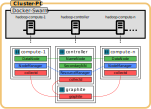
\includegraphics{./images/hadoopBenchmarkArch.png}
    \caption[High"=Level"=Architektur von Hadoop"=Benchmark]
    {High"=Level"=Architektur von Hadoop"=Benchmark.
        Entnommen aus \cite{abb:hadoopBenchmarkArch}.}
    \label{fig:hadoopBenchmarkArchitecture}
\end{figure}

\autoref{fig:hadoopBenchmarkArchitecture} zeigt die grundlegende Architektur der Plattform, die mithilfe eines Docker"=Swarms auf mehreren \emph{Docker Machines} ein Cluster erstellt, auf denen dann in den Docker"=Containern das eigentliche Hadoop"=Cluster ausgeführt wird.
In Hadoop"=Benchmark werden mithilfe von Docker"=Machine und VirtualBox\footnote{\url{https://www.virtualbox.org/}} virtuelle Maschinen erstellt, die mit dem  Betriebssystem \emph{Boot2Docker} ausgestattet sind.
Boot2Docker ist eine leichtgewichtige Linux"=Distribution, auf der Docker bereits vorinstalliert ist \cite{DockerMachineGettingStartedVm}.
Jeder Hadoop"=Container enthält zudem das Tool \emph{collectd}\footnote{\url{https://collectd.org/}}, was das Monitoring des Containers auf Systemebene übernimmt und die Daten an den Graphite"=Container übermittelt.
Dadurch wird es möglich, eine beliebige Anzahl an voneinander unabhängigen Nodes auf einem physischen Computer ausführen zu können.
Auch ist es möglich, den Docker"=Machines einen beliebig großen Arbeitsspeicher zur Verfügung zu stellen.

Die Plattform Hadoop"=Benchmark enthält zudem einige Benchmark"=Anwendungen:

\begin{itemize}
    \item Hadoop Mapreduce Examples
    \item Intel HiBench\footnote{\url{https://github.com/intel-hadoop/HiBench}}
    \item \ac{SWIM} \footnote{\url{https://github.com/SWIMProjectUCB/SWIM}}
\end{itemize}

Eine Besonderheit bildet der SWIM"=Benchmark, welcher sehr Ressourcenintensiv ist und daher auf einem \emph{Single Node Cluster}, also einem kompletten Hadoop"=Cluster auf nur einem Computer, sehr zeitintensiv sein kann.
Der Intel HiBench"=Benchmark besteht aus Kategorien wie \emph{Machine Learning} oder Graphen, welche wiederum aus einen oder mehreren \emph{Workloads} bestehen, welche entsprechende Anwendungen bzw. Algorithmen auf dem Hadoop"=Cluster ausführen.
Einige der Hibench"=Workloads basieren auf den Mapreduce Examples, welche wiederum voneinander unabhängige Beispielanwendungen für Hadoop darstellen.

\subsection{In dieser Fallstudie verwendetes Setup}\label{sec:clusterFallstudie}

Da die Plattform Hadoop"=Benchmark mithilfe von Docker auf einem physischen PC sehr einfach ein komplettes Hadoop"=Cluster ausführen kann, wurde die Plattform für diese Fallstudie als Basis genutzt.
Da Docker und Hadoop vor allem für den Einsatz in einer Linux"=Umgebung entwickelt wurden, werden für die Fallstudie zwei Computer genutzt, auf denen das Cluster wahlweise auf einem oder auf beiden Hosts ausgeführt werden kann.
Zudem wird auf einem Host eine VM mit Windows 10 ausgeführt, das zum Ausführen des .NET"=Frameworks bzw. \sS benötigt wird.
Beide zum Einsatz kommenden Hosts sind jeweils mit einem Intel Core i5"=4570 @ 3,2 GHz x 4, 16 GB Arbeitsspeicher sowie einer SSD ausgestattet, auf der Ubuntu 16.04 LTS installiert ist.
Die Verbindung von Windows zu Linux auf beiden Hosts wird mithilfe von SSH"=Verbindungen umgesetzt.

\begin{figure}
    \includegraphics{./images/caseStudyHadoopSetup.pdf}
    \caption[In der Fallstudie verwendetes Cluster"=Setup]
    {In der Fallstudie verwendetes Cluster"=Setup.
        Grün: \ac{HDFS}, Blau: YARN, Rot: Graphite.}
    \label{fig:caseStudyHadoopSetup}
\end{figure}

\todo{Irgendwo erwähnen, wie Docker-Container aufeinander aufbauen}
Die beiden Abbildungen \autoref{fig:hadoopBenchmarkArchitecture} und \autoref{fig:caseStudyHadoopSetup} zeigen bereits den großen Hauptunterschied zwischen der Plattform und dem hier verwendeten Cluster"=Setup.
Da durch die Nutzung von virtuellen Maschinen ein zusätzlicher Ressourcenbedarf entsteht, wird im hier verwendeten Setup darauf verzichtet.
Durch die Ausführung der Docker"=Container des Hadoop"=Clusters direkt auf dem Host stehen dem Cluster mehr Ressourcen zur Verfügung.
Zudem wird es mithilfe von von \emph{Docker Swarm} so ermöglicht, das Hadoop"=Cluster auf beiden Hosts auszuführen.
Im konkreten Setup werden dabei Graphite, der Hadoop"=Controller sowie vier Hadoop"=Nodes auf dem Host1, sowie zwei weitere, optionale Nodes auf Host2 ausgeführt.
Weitere Anpassungen des verwendeten Setups bestehen \uA darin, dass der \ac{TLS} von Hadoop ebenfalls gestartet wird.
Zudem wurden einige Einstellungen von Hadoop so angepasst, dass defekte Nodes schneller erkannt werden.

Zum Ausführen der Windows"=VM auf Host2 wird VirtualBox 5.2 verwendet.
Zum Abrufen von Daten mithilfe der REST"=API von Hadoop über die SSH"=Verbindungen wird \emph{curl}\footnote{\url{https://curl.haxx.se/}} genutzt.
Zum Ausführen des Hadoop"=Clusters wird Docker in der Version 18.03 CE genutzt.

Um die in dieser Fallstudie benötigten Befehle einfach ausführen zu können, wurden zwei eigene Scripte erstellt, welche zum Teil auf den bestehenden Scripten der Plattform aufbauen.
Das Setup"=Script dient für folgende Zwecke:

\begin{itemize}
    \item Starten und Beenden des Clusters
    \item Starten und Beenden einzelner Hadoop"=Nodes
    \item Hinzufügen und Entfernen der Netzwerkverbindung des Docker"=Containers eines Hadoop"=Nodes
    \item Ausführen von eigenen Befehlen auf dem Docker"=Container des Hadoop"=Controllers
    \item Erstellen des Hadoop"=Docker"=Images
\end{itemize}

Das zweite erstellte Script dient ausschließlich zum Starten der Benchmarks.
Dazu werden die in der Plattform bereits enthaltenen Start"=Scripte aufgerufen, die für das konkrete Setup angepasst wurden.

    \chapter{Entwicklung des Testsystems}
\label{ch:model}

Um die in \cref{ch:caseStudy} beschriebene Fallstudie durchführen zu können, wurde zunächst TestingHadoop mithilfe des \gls{ss}"=Frameworks entwickelt.
Das Testsystem bildet \uA vereinfacht die für die Fallstudie relevanten YARN"=Komponenten ab und besteht aus den drei im Folgenden beschriebenen, architektonischen Schichten.

Da für die Fallstudie \cite{Eberhardinger2018} ebenfalls das hier beschriebene TestingHadoop genutzt wurde, wurden entsprechende Teile der Beiträge dieses Kapitels dort bereits publiziert.

\section{Grundlegende Architektur des Testmodells}
\label{sec:modelArchitecture}

Um Hadoop mit der Selfbalancing"=Komponente mit den in \cref{sec:requirements} beschriebenen Anforderungen prüfen zu können, wird mithilfe des \gls{ss}"=Frameworks ein vereinfachtes Modell der relevanten \gls{YARN}"=Komponenten entwickelt.
Dieses \gls{YARN}"=Modell wird mithilfe des Treibers mit dem realen Cluster verbunden, was durch hierfür entwickelte Scripte gesteuert wird.
Daraus resultiert folgende Drei"=Schichten"=Architektur für das gesamte Testmodell:

\begin{figure}[h]
    \includegraphics[width=0.6\columnwidth]{./resources/modelArchitecture.pdf}
    \caption{Grundlegende Architektur des Testmodells}
    \label{fig:modelArchitecture}
\end{figure}

Das \gls{YARN}"=Modell stellt die oberste Schicht des Testmodells dar.
Es bildet das Kernstück dieser Fallstudie, da dieses Modell mit den hierin abgebildeten \gls{YARN}"=Komponenten und Komponentenfehlern, dem Controller und dem Oracle direkt im Rahmen des modellbasierten Testens mit \gls{ss} interagiert.
Folgende Komponenten sind im \gls{YARN}"=Modell enthalten:

\begin{description}
    \item [Controller] \hfill \\
        Steuert den Ablauf einer Testausführung und das Zusammenspiel zwischen den Komponenten des \gls{YARN}"=Modells.
    \item [Relevante \gls{YARN}"=Komponenten und Eigenschaften] \hfill \\
        Bilden die grundlegende Architektur von Hadoop \gls{YARN} ab.
        Implementiert wurden in dieser Fallstudie die Nodes, Anwendungen, \glspl{Attempt} und \gls{Container} mit den jeweils relevanten Eigenschaften zur Durchführung der Fallstudie.
    \item [Komponentenfehler der \gls{YARN}"=Komponenten] \hfill \\
        Bilden die bei den \glspl{Test} zu injizierenden Komponentenfehler der jeweiligen \gls{YARN}"=Komponenten.
    \item [Oracle] \hfill \\
        Validiert die in Form von Constraints in den jeweiligen \gls{YARN}"=Komponenten implementierten Anforderungen.
    \item [Client] \hfill \\
        Dient zum starten und beenden von Benchmarks im Cluster.
    \item [Benchmark"=Controller] \hfill \\
        Enthält das Transitionssystem zur Auswahl der Benchmarks und steuert diese.
\end{description}

Die Verbindung zwischen dem \gls{YARN}"=Modell und dem realem Cluster bildet der Treiber.
Er besteht aus folgenden Komponenten:

\begin{description}
    \item [Parser] \hfill \\
        Verarbeitet die Monitoring"=Ausgaben vom realen Cluster und konvertiert diese für die Nutzung im \gls{YARN}"=Modell.
    \item [Connector] \hfill \\
        Abstrahiert die Verbindung zum realen Cluster und die dabei auszuführenden Befehle.
    \item [SSH"=Verbindung]  \hfill \\
        Stellt die Verbindung zum realen Cluster her.
\end{description}

Der Parser wird hierbei nur zur Durchführung des Monitoring benötigt und nutzt wiederum den Connector zum abrufen der Daten.
Andere Befehle und Zugriffe auf das reale Cluster, wie \zB das Injizieren von Komponentenfehlern, werden direkt mithilfe des Connectors durchgeführt.

In allen Komponenten des Modells werden zudem mithilfe des Frameworks log4net\footnote{\url{https://logging.apache.org/log4net/}}, Logausgaben durchgeführt.
Dies betrifft vor allem das Monitoring (vgl. \cref{subsec:yarnComponentInterface}), aber auch weitere Informationen wie zur Validierung der Constraints (vgl. \cref{subsec:oracleImpl}) oder reine Debug"=Informationen.
All diese Informationen werden im Programmlog zusammengefasst, welches auch zur Auswertung der ausgeführten \glspl{Test} dient.
Zu Analysezwecken im Fehlerfall wird zudem jede Kommunikation der SSH"=Verbindung in einem eigenen Log, dem SSH"=Log, abgespeichert (vgl. \cref{subsec:sshConnection}).

Die Implementierung des \gls{YARN}"=Modells wird in \cref{sec:yarnModel,sec:benchmarkController} beschrieben, die Implementierung des Treibers in \cref{sec:sshDriver}.
Die Umsetzung des realen Clusters wird in \cref{sec:realCluster} beschrieben.


\section{Implementierung des \acs{YARN}"=Modells}
\label{sec:yarnModel}

Das implementierte \ac{YARN}"=Modell besteht, wie bereits in \autoref{sec:modelArchitecture} gezeigt, aus fünf Komponenten und den Komponentenfehlern der hier relevanten \ac{YARN}"=Komponenten.
Die vier implementierten \ac{YARN}"=Komponenten sind die Anwendungen, ihre Attempts und Container, sowie die Nodes.
Zudem wurde eine Klasse implementiert, die zur Repräsentation des \ac{RM} dient, welche zudem auch als Controller im Rahmen des Testens mit \ac{ss} dient.
Einen Überblick über das Zusammenspiel des implementierten \ac{YARN}"=Modells gibt folgendes Klassendiagramm:

\begin{figure}[h]
    \includegraphics{./images/yarnModel_ls_MA.pdf}
    \caption[Grundlegender Aufbau des \acs{YARN}"=Modells]
        {Grundlegender Aufbau des \acs{YARN}"=Modells.
        Assoziationen und weitere Verbindungen zum Treiber und \acs{ss} sind hier aus Gründen der Übersichtlichkeit nicht dargestellt.}
    \label{fig:yarnModelClassDiagram}
\end{figure}

Im Folgenden werden zunächst die gemeinsam genutzten Bestandteile des \ac{YARN}"=Modells erläutert, welche nicht im Klassendiagramm enthalten sind, anschließend die fünf Komponenten des Modells, sowie die implementierten Komponentenfehler und basierend auf den in \autoref{sec:requirements} definierten Anforderungen implementierten Constraints.

\subsection{Gemeinsam genutzte Bestandteile des \acs{YARN}"=Modell}
\label{sec:yarnModelBasics}

\todo{Multihost-Mode irgendwo erklären}
\todo{irgendwo noch constraints einbauen}

\subsection{Relevante \acs{YARN}"=Komponenten}
\label{sec:yarnComponents}

\begin{figure}[h]
    \includegraphics[width=\columnwidth]{./images/yarnComponents.pdf}
    \caption[Für die Fallstudie relevante, implementierte \acs{YARN}"=Komponenten mit den wichtigsten Eigenschaften und Methoden]
        {Für die Fallstudie relevante, implementierte \acs{YARN}"=Komponenten mit den wichtigsten Eigenschaften und Methoden.
        Dies sind alle für die spätere Durchführung und zur Ausgabe des Zustandes (vgl. \autoref{sec:dataOrganisation}) wichtigen Eigenschaften und Methoden.
        Aus Gründen der Übersichtlichkeit sind die implementierten Komponentenfehler, einige der \texttt{IYarnReadable} bereitgestellten, relevanten Eigenschaften und Methoden, sowie die Klasse \texttt{YarnAppContainer} nicht aufgeführt.}
    \label{fig:yarnComponentsClassDiagram}
\end{figure}

\subsection{Implementierung des Clients}
\label{sec:yarnClient}

\subsection{Implementierung des Controllers}
\label{sec:yarnController}

\subsection{Implementierung des Oracles}
\label{sec:oracleImpl}

\todo{ab hier alte struktur!}

\begin{figure}
    \includegraphics[width=\columnwidth]{./images/yarnModel.png}
    \caption[Aufbau des YARN"=Modells]
    {Aufbau des YARN"=Modells.
        Das Modell wurde mithilfe des Klassendiagramm"=Designers in Visual Studio 2017 visualisiert.
        Daher werden Assoziationen mit höherer Multiplizität als 1, die daher mithilfe von \texttt{List<T>} umgesetzt wurden (\zB \texttt{YarnApp.Attempts}) im Diagramm nicht als Assoziationen zwischen den Klassen angezeigt.}
    \label{fig:yarnModel}
\end{figure}

\autoref{fig:yarnModel} beschreibt im Grunde bereits das gesamte von \sS verwendete YARN"=Modell.
Enthalten sind alle hier relevanten Komponenten sowie deren Eigenschaften.
Als Eigenschaften wurden die Daten aufgenommen, welche mithilfe von Shell"=Kommandos bzw. mithilfe der REST"=API von YARN ermittelt werden können.

\subsection{Modellierte YARN"=Komponenten}%\label{sec:yarnComponents}

Die abstrakte Basisklasse \texttt{YarnHost} stellt die Basis für alle Hosts des Clusters dar, also dem \texttt{YarnController} mit dem \ac{RM}, und dem \texttt{YarnNode}, was einen Node darstellt, auf dem die Anwendungen bzw. deren Container ausgeführt werden.
Die abstrakte Eigenschaft \texttt{YarnHost.HttpPort} dient als Hilfs"=Eigenschaft, da Controller und Nodes unterschiedliche Ports für die Weboberfläche nutzen, deren URL mit Port in der Eigenschaft \texttt{YarnHost.HttpUrl} abrufbar ist.
Sie wird daher vom Controller bzw. Node mit dem entsprechenden Port versehen.

Die mithilfe von \texttt{YarnApp} dargestellten Anwendungen werden mithilfe des \texttt{Bench"-Controller}s (vgl. \autoref{sec:appImplementation}) eines Clients (entsprechend repräsentiert durch die gleichnamige Klasse) gestartet.
Jeder Client kann nur eine Anwendung ausführen, daher gibt es die Möglichkeit, mehrere Clients zum Starten von mehreren gleichzeitig ausgeführten Anwendungen zu nutzen.
Die Anwendungen selbst enthalten neben grundlegenden Daten wie \zB den Namen auch einige Daten zum Ressourcenbedarf (Speicher und CPU).
Zwar gibt Hadoop nicht direkt die zu der Anwendung gehörigen Job"=Ausführungen an, allerdings können diese mithilfe der \texttt{YarnApp.AppId} sehr einfach ermittelt werden und dann in der Liste \texttt{YarnApp.Attempts} gespeichert werden.
Das Feld \texttt{YarnApp.IsKillable} gibt an, ob die Ausführung der Anwendung mit den aktuellen Daten im Modell durch den Komponentenfehler \texttt{YarnApp.KillApp} abgebrochen werden kann.
Abhängig ist das durch \texttt{YarnApp.FinalStatus}, was angibt, ob eine Anwendung erfolgreich oder nicht erfolgreich ausgeführt wurde oder die Ausführung noch nicht abgeschlossen ist (durch \texttt{EFinalStatus.UNDEFINED}).
Um die Komponentenfehler zu aktivieren bzw. bei Bedarf auch wieder zu deaktivieren, besitzen \texttt{YarnNode} und \texttt{YarnApp} jeweils die Eigenschaft \texttt{FaultConnector}, mit der auf den benötigten Connector zugegriffen werden kann.

Jede Ausführung \texttt{YarnAppAttempt} hat eine eigene ID und kann einer Anwendung zugeordnet werden.
Genau wie bei den Anwendungen selber wird hier direkt der Node gespeichert, auf welchem der \ac{AppMstr} ausgeführt wird und einen eigenen Container bildet, dessen ID direkt gespeichert wird.
Container (dargestellt durch \texttt{YarnAppContai"-ner}) existieren in Hadoop nur während der Laufzeit eines Programmes und enthalten nur wenige Daten, darunter ihr ausführender Node.
Jede Anwendung, deren Ausführungen und deren Container enthalten zudem den derzeitigen Status, ob die Komponente noch initialisiert wird, bereits ausgeführt wird oder beendet ist.
\texttt{EAppState.NotStartedYet} dient als Status, den es nur im Modell gibt und angibt, dass die Anwendung im späteren Verlauf der Testausführung gestartet wird.

Alle vier YARN"=Kernkomponenten implementieren das Interface \texttt{IYarnReadable}, was angibt, dass die Komponente ihren Status aus Hadoop ermitteln kann.
Entsprechend wird in allen Komponenten die Methode \texttt{ReadStatus()} implementiert, in welchem mithilfe des angegebenen Parsers auf den SSH"=Treiber zugegriffen werden kann und die Komponenten im Modell so ihre eigenen Daten aus dem realen Cluster ermitteln können.
Da die REST"=API ermöglicht, alle Daten auch über die reinen Listen zu erhalten anstatt ausschließlich über die Detailausgabe, besteht auch im Modell mithilfe der Eigenschaft \texttt{IsRequireDetailsParsing} das Ermitteln der Daten so einzustellen, dass die übergeordnete YARN"=Komponente bereits alle Daten ermittelt und der Untergeordneten zum Speichern (mittels \texttt{SetStatus()}) übergibt.
Als Basis dazu dient der \texttt{YarnController}, der dafür die Daten aller Anwendungen ausliest, die wiederum die Daten ihrer Ausführungen auslesen, welche dann die Daten ihrer Container auslesen und den Komponenten zum Speichern übergeben.

\subsection{Implementierung der Komponentenfehler}%\label{sec:implementedFaults}

Die Felder \texttt{YarnNode.NodeConnectionError} und \texttt{YarnNode.NodeDead} definieren die Komponentenfehler, wenn ein Node seine Netzwerkverbindung verliert bzw. beendet wird.
Die aus den Komponentenfehlern resultierenden Effekte werden in den dafür implementierten geschachtelten Klassen definiert.
\autoref{lst:faultInjection} zeigt beispielhaft die Implementierung und Injizierung des \texttt{NodeDead}"=Komponentenfehlers mithilfe des für den Node verwendeten \texttt{CmdConnector} (vgl. \autoref{sec:implementedConnectors}).
Die Injizierung des \texttt{NodeConnectionError}"=Komponentenfehlers und die Aufhebung beider Komponentenfehler sind analog implementiert.

\lstinputlisting[label=lst:faultInjection,
caption={[Injizierung eines Komponentenfehlers]
    Injizierung eines Komponentenfehlers (gekürzt).
    Sollte der Node nicht beendet werden, wird die Injizierung einmalig erneut versucht. \texttt{CmdConnector.Faulting} ist der für Komponentenfehler verwendete Connector.},
float,style=cs]
{./listings/faultInjectionExample.cs}

\subsection{Fehlerüberprüfung}%\label{sec:FaultTesting}

Um zu prüfen, ob sich das reale Cluster nach der Aktivierung bzw. Deaktivierung eines Komponentenfehlers korrekt rekonfiguriert, werden \emph{Constraints} genutzt.
\todo{Verweis zu Anforderungen}
Diese richten sich nach den funktionalen Anforderungen des Systems und prüfen, ob diese weiterhin eingehalten werden.
Da die funktionalen Anforderungen bei jeder YARN"=Komponente unterschiedlich sind, wurden diese mithilfe der Eigenschaft \texttt{IYarnReadable.Constraints} für jede Komponente einzeln definiert.
\autoref{lst:constraintDefinition} zeigt die Definition der Constraints für \texttt{YarnApp}, bei der die Anforderungen 1 und 3 eine Rolle spielen.
In jeder Komponente sind nur die funktionalen Anforderungen als Constraints implementiert, die für diese Komponente auch relevant sind.
Daher finden sich die beiden Anforderungen 2 und 4 nicht in der Klasse \texttt{YarnApp} wieder, letztere dafür aber \zB in \texttt{YarnNode}.

\lstinputlisting[label=lst:constraintDefinition,
caption={[Definition der Constraints in YarnApp]
    Definition der Constraints in \texttt{YarnApp}},
float,style=cs]
{./listings/constraints.cs}

Geprüft werden die Constraints im Anschluss an das Monitoring der einzelnen YARN"=Komponenten.
Wenn dabei die Bedingungen einer funktionalen Anforderungen nicht erfüllt werden, wird von den Constraints \texttt{false} zurückgegeben und so erkannt, dass bei dieser Komponente ein Fehler von Hadoop nicht selbst korrigiert wurde.
Die ID der Komponente wird daher entsprechend ausgegeben bzw. in der Logdatei gespeichert.
Zwar wäre es hier auch möglich gewesen, ähnlich wie in den Modellen der anderen Fallstudien, die mit dem \sS-Framework entwickelt wurden, eine Exception zu werfen, jedoch wurde hier darauf verzichtet, damit immer die Daten aller Komponenten geprüft werden können.
Dadurch kann erkannt werden, wenn mehrere Komponenten nicht den funktionalen Anforderungen entsprechen.

Nach der Überprüfung der Constraints wird abschließend geprüft, ob es dem Cluster möglich ist, sich überhaupt rekonfigurieren zu können.
Dies wird dadurch realisiert, dass geprüft wird, ob mindestens ein Node noch aktiv ist.
Dabei wird jedoch nicht der interne Fehlerstatus in \texttt{YarnNode.IsActive} oder \texttt{YarnNode.IsConnected} geprüft, sondern der beim Monitoring vom Cluster zurückgegebene \texttt{YarnNode.State}.
Nur wenn dieser den Wert \texttt{ENodeState.Running} hat, ist der Node aktiv und kann Anwendungen ausführen.
Das reale Hadoop"=Cluster kann sich somit nicht mehr rekonfigurieren und neue Container allokieren bzw. in der Ausführung befindliche Anwendungen und ihre Komponenten umverteilen, wenn kein Node den Wert \texttt{ENodeState.Running} hat.
\todo{Verweis auf Abschnitt, wo implementierung der Simulation genauer erklärt wird}
Kommt es zu diesem Fall, wird dies analog zu den Constraints ebenfalls ausgegeben und in der Logdatei vermerkt und die Ausführung des Simulationsschrittes fortgeführt, da die Daten aller Yarn"=Komponenten erst nach Abschluss der Simulation eines Schrittes ausgegeben werden.
Somit kann im Fehlerfall einfacher ermittelt werden, wie der Systemzustand zum Zeitpunkt des Fehlers war.


\section{SSH-Treiber}\label{sec:sshDriver}

Im Einführungstext zu diesem Kaptiel wurde bereits auf den grundlegenden Aufbau des Treibers eingegangen, der aus den drei einzelnen Komponenten Parser, Connector und der eigentlichen SSH-Verbindung besteht. Der Parser selbst besteht neben dem eigentlichen Parser zudem aus Datenhaltungs-Klassen für die relevanten YARN-Komponenten. Sie sind außerdem so aufgebaut, dass sie für beide hier implementierten Parser bzw. Connectoren für die Kommandozeilen-Befehle und die REST-API genutzt werden können.

\subsection{Integration im Modell}\label{sec:modelIntegration}

Hadoop besitzt zwei primäre Wege, um die Daten vom \ac{RM} bzw. dem \ac{TLS} ausgeben zu können. Dies ist zum einen die Kommandozeile, mithilfe der die Daten vom \ac{RM} und vom \ac{TLS} kombiniert ausgegeben werden, und die REST-API. Die benötigten Befehle für die Kommandozeile und deren Ausgaben sind in \autoref{app:hadoopCmds}, die für die REST-API benötigten URLs und deren Rückgaben in \autoref{app:hadoopRestApi} gelistet. Auf beiden Wegen können \uA die Daten zu folgenden Komponenten ausgegeben werden \cite{HadoopYarnTlServer271,HadoopYarnCmds271,HadoopRmApi271,HadoopNmApi271}:

\begin{description}
    \item[Anwendungen] als nach dem Status gefilterte Liste oder der Report einer Anwendung
    \item[Ausführungen] als Liste aller Ausführungen einer Anwendung oder der Report einer Ausführung
    \item[Container] als Liste aller Container einer Ausführung oder der Report eines Containers
    \item[Nodes] als Liste aller Nodes oder der Report eines Nodes
\end{description}

Zur Integration des Treibers wurden daher entsprechende Interfaces entwickelt, über die das Modell auf den eigentlichen Treiber zugreifen kann.

Die vier Interfaces \texttt{IApplicationResult}, \texttt{IAppAttemptResult}, \texttt{IContainerResult} und \texttt{INodeResult} dienen der Übergabe der geparsten Daten der einzelnen Komponenten an die korrespondierenden Komponenten im \sS-Modell. Sie enthalten jeweils alle relevanten Daten, die von Hadoop über die Kommandozeile oder die REST-API ausgegeben werden. Alle vier Interfaces implementieren zudem \texttt{IParsedComponent}, welches wiederum als Basis für die Übergabe der ausgelesenen Daten an \texttt{IYarnReadable.SetStatus()} im Modell dient.

Das Interface \texttt{IHadoopParser} dient als Einbindung des Parsers im Modell mithilfe von \texttt{IYarnReadable.Parser} und enthält für jede der acht relevanten Ausgaben von Hadoop entsprechende Methodendefinitionen.

Beim Interface \texttt{IHadoopConnector}, das im Modell den Connector über die \texttt{Fault"-Connector}-Eigenschaften von \texttt{YarnApp} und \texttt{YarnNode} einbindet, besitzt ebenfalls für jede der acht Datenrückgaben entsprechende Deklarationen, für Ausführungen und Container dabei jeweils vom \ac{RM} (\ac{NM} für Container) und vom \ac{TLS}. Auf die Nutzung des \ac{TLS} zum Ermitteln der Daten zu Anwendungen wird verzichtet. Dies liegt darin begründet, dass bei Nutzung der REST-API des \ac{RM} neben den vom \ac{TLS} bereitgestellten Daten einige weitere Informationen zu den Anwendungen ausgegeben werden \cite{HadoopRmApi271,HadoopYarnTlServer271}. Das Connector-Interface enthält darüber hinaus Deklarationen, um die im Modell implementierten Komponentenfehler im realen Cluster zu steuern und Anwendungen starten zu können. Architektonisch ist der Treiber zudem so aufgebaut, dass das Modell keine Kontrolle über den vom Parser benötigten Connector besitzt und die SSH-Verbindung ausschließlich vom Connector gesteuert werden kann.

\subsection{Implementierte Parser}\label{sec:implementedParsers}

Da die Daten für die relevanten Komponenten auf zwei Arten ermittelt werden können und unterschiedliche Ausgaben erzeugen, wurden auch für beide Arten ein Parser (\texttt{CmdParser} und \texttt{RestParser}) entwickelt. Da der Parser von außerhalb keinerlei weitere Informationen erhält außer der ID der zu parsenden YARN-Komponente, ist der Parser selbst dafür verantwortlich, die Daten von einem korrespondierenden Connector zu erhalten. Daher muss zur Initialisierung eines Parsers zunächst der korrespondierende Connector initialisiert werden. Da für die Nutzung der REST-API zum Teil die IDs der übergeordneten YARN-Komponenten ebenfalls nötig sind, ist der \texttt{RestParser} zudem auch dafür verantwortlich, die entsprechenden IDs zu ermitteln, bei der Nutzung der Kommandozeile reichen aufgrund der Befehlsstruktur die IDs der Komponenten selbst.

Die konkreten Implementierungen der auf \texttt{IParsedComponent} basierenden Übergabe"=Interfaces können ebenfalls als Bestandteil des Parsers angesehen werden. Sie wurden zudem so implementiert, dass sie für beide entwickelten Parser genutzt werden können.

Der grundlegende Ablauf ist bei jedem Parsing-Vorgang gleich. Zunächst werden, sofern benötigt, die benötigten YARN-Komponenten-IDs ermittelt und die Rohdaten mithilfe des Connectors von Hadoop abgefragt. Auch vom Parser wird dabei analog zum Modell das Abrufen der Daten ausschließlich mithilfe des Interfaces \texttt{IHadoopConnector} durchgeführt. Anschließend findet das eigentliche Parsing der Ausgabe von Hadoop statt, deren Daten direkt in der für die YARN-Komponente vorgesehene \texttt{IParsed"-Compo"-nent}-Implementierung gespeichert werden. Da Hadoop über die Kommandozeile die Daten in keinem standardisierten Format zurückgibt, wurde das Parsing der Rohdaten von Hadoop beim \texttt{CmdParser} in eigenem Code mithilfe von \emph{Regular Expressions} realisiert. Bei der Nutzung der REST-API werden die Daten dagegen im JSON-Format zurückgegeben \cite{HadoopYarnTlServer271,HadoopRmApi271,HadoopNmApi271}, wodurch diese mithilfe des \emph{Json.NET}-Frameworks\footnote{\url{https://www.newtonsoft.com/json}} deserialisiert und direkt als die entsprechende \texttt{IParsedComponent}-Implementierung gespeichert werden. Da \ac{RM} und \ac{TLS} verschiedene Daten einer YARN-Komponente ausgeben, werden, sofern nötig, \ac{RM} und \ac{TLS} abgefragt und die dabei ermittelten Daten zusammengeführt.

Eine erste Besonderheit bildet zudem das Abrufen und Parsen der Report-Daten mittels REST-API. Da die Listen hierbei als Array der einzelnen Reports zurückgegeben werden \cite{HadoopYarnTlServer271,HadoopRmApi271,HadoopNmApi271}, wird beim Parsen eines Ausführungs- oder Container-Reports die komplette Liste abgerufen und geparst. Anschließend wird in dieser Liste basierend auf der ID die benötigte Komponente herausgefiltert.

Die zweite Besonderheit bei der Nutzung der REST-API liegt darin, dass die Daten zu derzeit ausgeführten Container ausschließlich vom \ac{NM}, auf dem der Container ausgeführt wird, zurückgegeben werden können \cite{HadoopRmApi271,HadoopNmApi271}. Daher werden zur Ermittlung der Container-Listen alle Nodes abgefragt und anschließend die benötigten Container gefiltert.

Die geparsten Daten werden abschließend als das für die YARN-Komponente vorgesehene Interface zurückgegeben, was anschließend im Modell zum Speichern der Daten genutzt werden kann.

\subsection{Implementierte Connectoren}\label{sec:implementedConnectors}

Für die beiden Parser wurden die beiden korrespondieren Connectoren \texttt{CmdConnector} und \texttt{RestConnector} entwickelt. Während der Connector für die REST-API nur über eine SSH-Verbindung verfügt, besteht beim Connector für die Kommandozeile die Möglichkeit, mehrere einzelne SSH-Verbindungen zu nutzen. Dies ist damit begründet, dass zum Steuern der Komponentenfehler, was nur über die Kommandozeile möglich ist, eine eigene SSH-Verbindung genutzt wird. Zum Starten von Anwendungen besteht zudem die Möglichkeit, eine beliebige Anzahl an einzelnen SSH-Verbindungen aufzubauen, damit mehrere Anwendungen parallel gestartet werden können. Da die Daten der einzelnen YARN-Komponenten in der Fallstudie bevorzugt mithilfe der REST-API ermittelt werden, kann die dafür vorgesehene SSH-Verbindung des \texttt{CmdConnector} deaktiviert werden.

Da über die Kommandozeile die Befehle für die Daten vom \ac{TLS} die gleichen wie für die Daten vom \ac{RM} sind \cite{HadoopYarnTlServer271,HadoopYarnCmds271}, sind beim \texttt{CmdConnector} die \ac{TLS}-Methoden von geringer Bedeutung und nutzen daher ebenfalls die \ac{RM}-Methoden.

Der Connector ist beim Abrufen der Daten dafür zuständig, die dafür notwendigen Befehle auszuführen. Während dies für die Kommandozeilen-Befehle die entsprechenden Hadoop-Befehle sind, wird dies zum Abrufen der Daten über die REST-API mithilfe des Tools \emph{curl} durchgeführt. Die dabei zurückgegebenen Daten werden vom Connector ohne Verarbeitung zurückgegeben und können dann vom Parser verarbeitet werden.

Beim Steuern der Komponentenfehler wird vom Connector das für die Fallstudie entwickelte Start-Script verwendet. Nach dem eigentlichen Start bzw. Aufheben eines Komponentenfehlers wird vom Connector zudem überprüft, ob die Injizierung bzw. Aufhebung erfolgreich war. Während der Datenabruf sowie die Steuerung der Komponentenfehler synchron stattfindet, findet das Starten der Anwendungen asynchron und mithilfe des Benchmark-Scriptes statt. Da eine Ausführung einer YARN-Anwendung längere Zeit in Anspruch nehmen kann, wird dadurch die Ausführung von \sS nicht behindert und es können mehrere Anwendungen parallel ausgeführt werden.

\subsection{SSH-Verbindung}\label{sec:sshConnection}

Die SSH-Verbindung selbst ist der einzige Bestandteil des Treibers, welches kein entsprechendes Interface benötigt, die SSH-Verbindung wird ausschließlich vom Connector genutzt. Realisiert wird die Verbindung mithilfe des Frameworks SSH.NET,\footnote{\url{https://github.com/sshnet/SSH.NET}} weshalb die SSH-Verbindung im Treiber nur entsprechende Funktionen zum Aufbauen, Nutzen und Beenden der Verbindung enthält.

Um die Verbindung mit dem Cluster-PC aufzubauen, ist zudem ein dort installierter SSH-Key nötig. Ein Kommando auf dem Cluster-PC kann mithilfe der Treiberkomponente synchron und asynchron ausgeführt werden.

\section{Umsetzung des realen Clusters}
\label{sec:realCluster}

Da mithilfe der Plattform Hadoop"=Benchmark ein komplettes Hadoop"=Cluster auf einem PC ausgeführt werden kann und dieses speziell für die Forschung entwickelt wurde, wurde die Plattform für diese Fallstudie als Basis genutzt
Da Docker und Hadoop vor allem für den Einsatz in einer Linux"=Umgebung entwickelt wurden, werden für die Fallstudie zwei physische Hosts genutzt, auf denen das Cluster wahlweise auf einem oder auf beiden Hosts ausgeführt werden kann.
Zudem wird auf einem Host eine VM mit Windows 10 ausgeführt, das zum Ausführen des .NET"=Frameworks bzw. \ac{ss} benötigt wird.
Beide zum Einsatz kommenden Hosts sind jeweils mit einem Intel Core i5"=4570 @ 3,2 GHz x 4, 16 GB Arbeitsspeicher sowie einer SSD ausgestattet, auf der Ubuntu 16.04 LTS installiert ist.
Die Verbindung von Windows zu Linux auf beiden Hosts wird mithilfe von SSH"=Verbindungen umgesetzt.
Um den Ressourcenbedarf durch die von docker"=machine erzeugten VMs zu reduzieren, werden die Docker"=Container direkt auf den physischen Hosts ausgeführt:

\begin{figure}[h]
    \includegraphics{./resources/caseStudyHadoopSetup.pdf}
    \caption[In der Fallstudie verwendetes Cluster"=Setup]
    {In der Fallstudie verwendetes Cluster"=Setup.
        Grün: \ac{HDFS}, Blau: YARN, Rot: Graphite.}
    \label{fig:caseStudyHadoopSetup}
\end{figure}

\todo{Irgendwo erwähnen, wie Docker-Container aufeinander aufbauen}
Durch die leicht veränderte Architektur stehen dem Cluster daher mehr Ressourcen zur Verfügung.
Zudem wird es mithilfe von von \emph{Docker Swarm} so ermöglicht, das Hadoop"=Cluster auf beiden Hosts auszuführen.
Neben der auf Host1 ausgeführten Basis des Clusters besteht die Möglichkeit, die auf Host2 ausgeführten Hadoop"=Nodes optional zum Cluster hinzuzufügen.
\todo{Basisanzahl Nodes erläutern}
Ein weiterer Unterschied zur originalen Plattform besteht darin, dass der Hadoop"=\ac{TLS} ebenfalls gestartet wird.
Zudem wurden einige Einstellungen von Hadoop so angepasst, dass defekte Nodes schneller erkannt werden.

Die Windows"=VM auf Host2 wird mithilfe von VirtualBox 5.2 ausgeführt.
Zum Abrufen von Daten mithilfe der REST"=API von Hadoop über die SSH"=Verbindungen wird \emph{curl}\footnote{\url{https://curl.haxx.se/}} 7.47 genutzt.
Zum Ausführen des Hadoop"=Clusters wird Docker in der Version 18.03 CE genutzt.

Um die in dieser Fallstudie benötigten Befehle einfach ausführen zu können, wurden zwei eigene Scripte erstellt, welche zum Teil auf den bestehenden Scripten der Plattform aufbauen.
Das Setup"=Script dient für folgende Zwecke:

\begin{itemize}
    \item Starten und Beenden des Clusters
    \item Starten und Beenden einzelner Hadoop"=Nodes
    \item Hinzufügen und Entfernen der Netzwerkverbindung des Docker"=Containers eines Hadoop"=Nodes
    \item Ausführen von eigenen Befehlen auf dem Docker"=Container des Hadoop"=Controllers
    \item Erstellen des Hadoop"=Docker"=Images
\end{itemize}

Das zweite erstellte Script dient ausschließlich zum Starten der Benchmarks.
Dazu werden die in der Plattform bereits enthaltenen Start"=Scripte aufgerufen, die für das konkrete Setup angepasst wurden.


    \chapter{Implementierung der Benchmarks}
\label{ch:benchmarks}

Neben dem \gls{YARN}"=Modell selbst sind auch die während der Testausführung genutzten \glspl{Anwendung} ein wichtiger Bestandteil des gesamten Testmodells.
Da Hadoop selbst sowie die Plattform Hadoop"=Benchmark bereits einige \glspl{Anwendung} und Benchmarks enthalten, konnten diese auch im Rahmen dieser Fallstudie genutzt werden.
Dazu wurde eine Auswahl an \glspl{Anwendung} in einem Transitionssystem in Form einer Markow"=Kette miteinander verbunden, mit dem die Ausführungsreihenfolge der einzelnen \glspl{Anwendung} basierend auf Wahrscheinlichkeiten bestimmt wird.
Verwaltet werden die implementierten Benchmarks mithilfe des Benchmark"=Controllers.

Da für die durchgeführte Fallstudie \cite{Eberhardinger2018} das für diese Fallstudie entwickelte Testmodell genutzt wurde, enthält es auch das hierfür entwickelte Transitionssystem.
Daher wurden Teile der Beiträge dieses Kapitels dort bereits publiziert.

\section{Übersicht möglicher Anwendungen}
\label{sec:appOverview}

Hadoop-Benchmark enthält bereits die Möglichkeit, unterschiedliche Benchmarks zu starten.
Folgende Benchmarks sind bereits in der Plattform integriert (vgl. \cref{sec:hadoopBenchmark}):

\begin{itemize}
    \item Hadoop"=Mapreduce"=Examples
    \item Intel HiBench
    \item \acrfull{SWIM}
\end{itemize}

Jede Benchmark enthält ein spezifisches Start"=Script, um die jeweiligen Benchmarks in einem Docker"=Container zu starten.
Dieser Container wird, abhängig vom \texttt{HostMode} (vgl. \cref{subsec:hostMode}), auf der Docker"=Machine des \gls{RM} oder direkt auf dem Host gestartet.
Da es in Docker"=Umgebungen \textit{best practice} ist, für jeden Einsatzzweck ein eigenes Image zu erstellen bzw. Container zu starten, werden für jede der drei Benchmark"=Suites eigene Container ausgeführt.
Um mehrere Benchmarks gleichzeitig ausführen zu können, wurden die Startscripte der Benchmarks zudem entsprechend angepasst.

\subsection{Mapreduce"=Examples}
\label{subsec:mapreduceExamples}

Die Hadoop"=Mapreduce"=Examples sind unterschiedliche und meist voneinander unabhängige Anwendungen, die beispielhaft für die meisten Anwendungsfälle in einem produktiv genutzten Cluster sind.
Die Examples sind Teil der Hadoop"=Installation und daher standardmäßig in jedem Hadoop"=Cluster verfügbar.
Einige der Anwendungen der Examples sind:

\begin{itemize}
    \item Generatoren für Text und Binärdaten, \zB \acrlong{rtw}
    \item Analysieren von Daten, \zB \acrlong{wc}
    \item Sortieren von Daten, \zB \acrlong{so}
    \item Ausführen von komplexen Berechnungen, \zB die Ausführung der \emph{Bailey-Borwein-Plouffe-Formel} \cite{Bailey1997} zur Berechnung einzelner Stellen von $\pi$
\end{itemize}

\subsection{Intel HiBench}
\label{subsec:hibench}

Intel HiBench\footnote{\url{https://github.com/intel-hadoop/HiBench/}} ist eine von Intel entwickelte Benchmark"=Suite mit \emph{Workloads} zu verschiedenen Anwendungszwecken mit jeweils unterschiedlichen einzelnen Anwendungen.
Die Suite enthielt anfangs nur wenige Anwendungen \cite{Huang2010}, wurde im Laufe der Zeit jedoch stetig um neue Anwendungen und auch Workloads erweitert.
Das zeigt sich auch darin, dass in Hadoop"=Benchmark die HiBench"=Version \mbox{2.2} integriert ist, die einen noch deutlich geringeren Umfang an Workloads und Anwendungen besitzt, wie \zB die aktuellere Version 7.
Aus diesem Grund wurde vor der Analyse der Anwendungen der HiBench"=Suite das Docker"=Image entsprechend auf Version 7 aktualisiert, um die in der Zwischenzeit hinzugefügten Workloads und Anwendungen der Suite nutzen zu können.
HiBench enthält damit folgende Workloads mit einer unterschiedlichen Anzahl an möglichen Anwendungen:

\begin{itemize}
    \item Micro"=Benchmarks (basierend auf den Examples und den Jobclient"=Tests)
    \item Maschinelles Lernen
    \item SQL/Datenbanken
    \item Websuche
    \item Graphen
    \item Streaming
\end{itemize}

\subsection{\glsentryshort{SWIM}}
\label{subsec:swim}

\gls{SWIM}\footnote{\url{https://github.com/SWIMProjectUCB/SWIM/}} ist eine aus 50 einzelnen Workloads bestehende Benchmark"=Suite.
Das besondere an \gls{SWIM} ist, dass die Suite im Rahmen der Studie \cite{Chen2012} entwickelt wurde, und dadurch anhand mehrerer tausend real ausgeführter \gls{MR}"=Jobs entwickelt wurde.
Die dabei enthaltenen Workloads stellen damit eine größere Vielfalt an ausgeführten Anwendungen und damit einen größeren Testumfang dar als vergleichbare Benchmarks \cite{SwimWikiHome}.

Bei der Ausführung auf dem in dieser Fallstudie verwendeten Cluster wurden jedoch nicht alle Workloads fehlerfrei ausgeführt.
Zudem wird in \cite{InriaTutorial} explizit erwähnt, dass die Ausführung auf einem Cluster auf einem Host sehr zeitintensiv ist, sofern die Workloads überhaupt ausgeführt werden können.
\gls{SWIM} ist außerdem für Benchmarks eines Clusters mit mehreren physischen Nodes ausgelegt, weshalb die Ausführung in dieser Fallstudie extrem viel Zeit benötigten würde.
Daher wurde die Nutzung des \gls{SWIM}"=Benchmarks nicht weiter verfolgt.

\subsection{Jobclient"=Tests}
\label{subsec:jobclient}

Ebenfalls im Installationsumfang von Hadoop enthalten sind die hier aufgrund ihres Dateinamens als Jobclient"=Tests bezeichneten Anwendungen.
Hauptbestandteil dieser Tests sind vor allem weitere, den Mapreduce"=Examples ergänzende, Benchmarks, welche das gesamte Cluster oder einzelne Nodes testen.
Der Fokus der Jobclient"=Tests liegt im Gegensatz zu den Examples nicht auf dem \gls{MR}- bzw. YARN"=Framework, sondern beim HDFS.
Da die Jobclient-Tests kein Teil von Hadoop"=Benchmark sind, wurde zur Ausführung der Jobclient"=Test zunächst ein eigenes Start"=Script analog zur Ausführung der Mapreduce"=Examples erstellt, damit diese ebenfalls im Rahmen der Plattform Hadoop"=Benchmark gestartet werden können.
Die Jobclient"=Tests enthalten \uA folgende Arten an Anwendungen:

\begin{itemize}
    \item HDFS"=Systemtests, \zB \texttt{SilveTest}
    \item Reine Lastgeneratoren, \zB \texttt{NNloadGenerator}
    \item Eingabe/Ausgabe"=Durchsatz"=Tests, \zB \texttt{TestDFSIO}
    \item DummyAnwendungen \acrlong{sl} und \acrlong{fl}
\end{itemize}


\section{Auswahl der verwendeten Anwendungen}\label{sec:appSelection}

Damit die Fallstudie die Realität abbilden kann, wurden von allen verfügbaren Anwendungen einige ausgewählt und in ein Transitionssystem in Form einer Markow"=Kette überführt.
Diese Kette definiert die Ausführungsreihenfolge zwischen den einzelnen Anwendungen.
Eine zufallsbasierte Markow"=Kette wurde aus dem Grund verwendet, dass auch in der Realität Anwendungen nicht immer in der gleichen Reihenfolge ausgeführt werden und daher auch in der Fallstudie eine unterschiedliche Ausführungsreihenfolge der Anwendungen gewährleistet werden soll.
Mithilfe der Festlegung eines bestimmten Seeds für den in der Fallstudie benötigten Pseudo"=Zufallsgenerator besteht bei Bedarf dennoch die Möglichkeit, einen Test mit den gleichen Anwendungen wiederholen zu können.

Einige der in \autoref{sec:appOverview} erwähnten Mapreduce Examples werden häufig als Benchmark verwendet.
Einige Beispiele dafür sind die Anwendungen \acl{so} und \texttt{grep} (ermittelt Anzahl von Regex"=Übereinstimmungen), die bereits im Referenzpapier zum MapReduce"=Algorithmus als Benchmarks verwendet wurden \cite{Dean2008}.
\acl{tsr} ist ebenfalls ein weit verbreiteter Benchmark, der die Hadoop"=Implementierung der standardisierten \emph{Sort Benchmarks}\footnote{\url{https://sortbenchmark.org/}} darstellt \cite{Graves2013}.
Ebenfalls als guter Benchmark dient die Anwendung \acl{wc}, mit der ein großer Datensatz stark verkleinert bzw. zusammengefasst wird und dient daher als gute Repräsentation für Anwendungsarten, bei denen Daten extrahiert werden \cite{Huang2010,Chen2012}.

Da in dieser Fallstudie ein realistisches Abbild der ausgeführten Anwendungen ausgeführt werden soll, ist es nicht sehr hilfreich, die einzelnen Übergangswahrscheinlichkeiten im Transitionssystem anzugleichen oder rein zufällig zu verteilen.
Einen realistischen Einblick, welche Anwendungs- und Datentypen in produktiv genutzten Hadoop"=Clustern genutzt werden, geben \uA \cite{Chen2012} und \cite{HadoopDataTypes}.
Auffällig ist hierbei, dass die meisten Anwendungen in einem Hadoop"=Cluster innerhalb weniger Sekunden oder Minuten abgeschlossen sind und/oder Datensätze im Größenbereich von wenigen Kilobyte bis hin zu wenigen Megabyte verarbeiten.
Zu einem ähnlichen Ergebnis kamen auch \citeauthor{Ren2013} in \cite{Ren2013} und folgerten daher, dass für kleine Jobs evtl. einfachere Frameworks abseits von Hadoop besser geeignet wären.
Die Autoren der Studie in \cite{HadoopDataTypes} bezeichneten Hadoop aufgrund ihrer Ergebnisse als \enquote{potentielle Technologie zum Verarbeiten aller Arten von Daten}, stellten aber eine ähnliche Vermutung an wie \citeauthor{Ren2013}, dass Hadoop primär Daten nutze, die auch mit \enquote{traditionellen Plattformen} verarbeiten werden könnten.

Basierend auf den Ergebnissen der Studien und der in den anderen Publikationen verwendeten Benchmark"=Anwendungen, wurden folgende Anwendungen der Mapreduce"=Examples und Jobclient"=Tests in das Transitionssystem übernommen:

\begin{itemize}
    \item Generieren von Eingabedaten für andere Anwendungen:
    \begin{itemize}
        \item Textdateien: \ac{rtw} und \ac{dfw}
        \item Binärdateien: \ac{rw} und \ac{tg}
    \end{itemize}

    \item Verarbeitung von Eingabedaten:
    \begin{itemize}
        \item Auslesen bzw. Zusammenfassen: \ac{wc} und \ac{dfr}
        \item Transformieren: \ac{so} für Textdaten und \ac{tsr} für Binärdaten
        \item Validierung: \ac{tms} und \ac{tvl} für die jeweiligen Sortier"=Anwendungen
    \end{itemize}

    \item Ausführen von Berechnungen:
    \begin{itemize}
        \item \acl{pi}\acused{pi}: Quasi-Monte-Carlo-Methode zur einfachen Berechnung von $\pi$ 
        \item \ac{pt}: Berechnung von Pentomino-Problemen
    \end{itemize}

    \item Dummy"=Anwendungen: \ac{sl} und \ac{fl}
\end{itemize}

Der Grund für die Berücksichtigung von mehreren gleichen bzw. ähnlichen Anwendungen für einige Kategorien liegt darin, dass die unterschiedlichen Anwendungen eine unterschiedliche Ausführungsdauer bzw. Datenrepräsentation (Text und Binär) repräsentieren.
So stehen die beiden \texttt{TestDFSIO}"=Varianten für eine umfangreichere Datennutzung, während die jeweils anderen Anwendungen einen kleineren Umfang repräsentieren.
Ähnlich verhält es sich bei den beiden Berechnungs"=Anwendungen, bei denen die \acl{pt}"=Anwendung die deutlich umfangreicheren Berechnungen durchführt.
\texttt{TestDFSIO} enthält zudem die Möglichkeit, Daten zu genieren und zu lesen, weshalb diese Anwendung in zwei Kategorien verwendet wurde.
Haupteinsatzzweck der Anwendung liegt vor allem darin, den Datendurchsatz des \ac{HDFS} zu testen.

Eine Besonderheit bilden die beiden Dummy"=Anwendungen.
Beide werden in dieser Fallstudie dafür genutzt, um zu simulieren, wenn auf dem Cluster \zB derzeit nichts ausgeführt wird, oder ein unerwarteter Fehler während der Ausführung auftaucht.
Daher können beide Anwendungen unabhängig von der derzeit ausgeführten Anwendung als nachfolgende Anwendung ausgewählt werden.
Als nachfolgende Anwendungen für die Dummy"=Anwendungen kommen nur Anwendungen in Betracht, welche ihrerseits keine Eingabedaten benötigen. Dies sind:

\begin{itemize}
    \item \acl{dfw}
    \item \acl{rtw}
    \item \acl{tg}
    \item \acl{rw}
    \item \acl{pi}
    \item \acl{pt}
\end{itemize}

\begin{table}
    \resizebox{\linewidth}{!}{\begin{tabular}{l|c|c|c|c|c|c|c|c|c|c|c|c|c|c}
    	             & \textit{dfw} & \textit{rtw} & \textit{tg} & \textit{dfr} & \textit{wc} & \textit{rw} & \textit{so} & \textit{tsr} & \textit{pi} & \textit{pt} & \textit{tms} & \textit{tvl} & \textit{sl} & \textit{fl} \\ \hline
    	\textit{dfw} &     .600     &     .073     &      0      &     .145     &      0      &      0      &      0      &      0       &    .073     &    .073     &      0       &      0       &    .018     &    .018     \\ \hline
    	\textit{rtw} &     .036     &     .600     &      0      &      0       &    .145     &    .036     &    .109     &      0       &    .036     &      0      &      0       &      0       &    .019     &    .019     \\ \hline
    	\textit{tg}  &      0       &     .036     &    .600     &      0       &      0      &      0      &      0      &     .255     &      0      &    .073     &      0       &      0       &    .018     &    .018     \\ \hline
    	\textit{dfr} &      0       &     .073     &      0      &     .600     &      0      &    .036     &      0      &      0       &    .145     &    .109     &      0       &      0       &    .018     &    .019     \\ \hline
    	\textit{wc}  &     .073     &     .109     &      0      &      0       &    .600     &      0      &    .073     &      0       &    .073     &    .036     &      0       &      0       &    .018     &    .018     \\ \hline
    	\textit{rw}  &      0       &     .073     &    .073     &      0       &      0      &    .600     &      0      &      0       &    .109     &    .109     &      0       &      0       &    .018     &    .018     \\ \hline
    	\textit{so}  &      0       &     .073     &    .036     &      0       &    .073     &    .036     &    .600     &      0       &    .073     &      0      &     .073     &      0       &    .018     &    .018     \\ \hline
    	\textit{tsr} &      0       &      0       &      0      &      0       &      0      &      0      &      0      &     .600     &    .109     &    .073     &      0       &     .182     &    .018     &    .018     \\ \hline
    	\textit{pi}  &     .145     &     .109     &      0      &      0       &      0      &      0      &      0      &      0       &    .600     &    .109     &      0       &      0       &    .018     &    .019     \\ \hline
    	\textit{pt}  &     .109     &     .109     &      0      &      0       &      0      &    .073     &      0      &      0       &    .073     &    .600     &      0       &      0       &    .018     &    .018     \\ \hline
    	\textit{tms} &      0       &     .145     &      0      &      0       &      0      &    .073     &      0      &      0       &    .036     &    .109     &     .600     &      0       &    .018     &    .019     \\ \hline
    	\textit{tvl} &     .073     &     .109     &      0      &      0       &      0      &      0      &      0      &      0       &    .109     &    .073     &      0       &     .600     &    .018     &    .018     \\ \hline
    	\textit{sl}  &     .167     &     .167     &    .167     &      0       &      0      &    .167     &      0      &      0       &    .167     &    .167     &      0       &      0       &      0      &      0      \\ \hline
    	\textit{fl}  &     .167     &     .167     &    .167     &      0       &      0      &    .167     &      0      &      0       &    .167     &    .167     &      0       &      0       &      0      &      0
    \end{tabular}}
    \caption
    {Verwendete Markov"=Kette für die Anwendungs"=Übergänge in Tabellenform.}
    \label{tab:transMatrix}
\end{table}

Für die in \autoref{tab:transMatrix} dargestellte Markow"=Kette der Übergänge zwischen den Anwendungen wurde neben den Ergebnissen aus den Studien zudem berücksichtigt, welche Anwendungen bestimmte Eingabedaten benötigen.
Dadurch wird sichergestellt, dass die für einige Anwendungen benötigten Eingabedaten immer vorhanden sind, da diese ebenfalls im Rahmen der Ausführung der Benchmarks generiert werden.
Anwendungen ohne Eingabedaten können dagegen fast jederzeit ausgeführt werden.


\section{Entwicklung des Benchmark"=Controllers}
\label{sec:benchmarkController}

Die im YARN"=Modell (vgl. \cref{sec:yarnModel}) implementierten Benchmarks und das zur Auswahl der Benchmarks entwickelte Transitionssystem bilden zusammen den Benchmark"=Controller.
Der Benchmark"=Controller wurde als eigene Klasse \texttt{BenchmarkController} im Modell implementiert und wird von den Clients genutzt, um die Auswahl der Benchmarks vorzunehmen.
Der Benchmark"=Controller verwaltet die implementierten Benchmarks und stellt diese den Clients zum Starten zur Verfügung.
Damit die Clients unabhängig voneinander sind, wird für jeden Client ein eigener Benchmark"=Controller instanziiert (vgl. \cref{subsec:yarnClient}).

\subsection{Implementierung von Benchmarks und Transitionssystem}
\label{subsec:appImplementation}

Die Benchmarks sind mithilfe der Klasse \texttt{Benchmark} implementiert.
Sie enthält alle zur Ausführung der Benchmarks benötigten Informationen und stellt diese der \texttt{BenchmarkController}"=Klasse bzw. dem Client bereit, um die Anwendung des Benchmarks zu starten.
Da mehrere Clients unabhängig voneinander agieren können müssen, erhält jeder Client ein spezifisches Unterverzeichnis im HDFS, in dem sich die Ein- und Ausgabeverzeichnisse für die von ihm gestarteten Anwendungen befinden.
Das muss auch bei der Definition der Startbefehle der Anwendungen berücksichtigt werden, weshalb hierfür entsprechende Platzhalter ersetzt werden müssen, wenn mithilfe der Methode \texttt{GetStartCmd()} der Start"=Befehl des Benchmarks zurückgegeben wird:

\begin{lstlisting}[label=lst:benchmarkClass,style=cs,
caption={[Wesentliche Methoden der Klasse Benchmark]
    Wesentliche Methoden der Klasse \texttt{Benchmark}}]
public class Benchmark
{
  public Benchmark(int id, string name, string startCmd,
     string outputDir, string inputDir)
  {
    _StartCmd = startCmd;
    _InDir = inputDir;
    HasInputDir = true;
  }
  
  public string GetStartCmd(string clientDir = "")
  {
    var result = _StartCmd
       .Replace(OutDirHolder, GetOutputDir(clientDir))
       .Replace(InDirHolder, GetInputDir(clientDir));
    if(result.Contains(BaseDirHolder))
      result = ReplaceClientDir(result, clientDir);
    return result;
  }
}
\end{lstlisting}

Die im Modell enthaltenen Benchmarks sind als Array in \texttt{BenchmarkController} gespeichert.
Hierbei werden mithilfe der Holder"=Variablen, die in \texttt{GetStartCmd()} ersetzt werden, die Startbefehle der Anwendungen definiert:

\begin{lstlisting}[label=lst:benchmarkDefinition,style=cs,
caption={[Definition der verfügbaren Benchmarks im BenchmarkController]
    Definition der verfügbaren Benchmarks im \texttt{BenchmarkController} (gekürzt)}]
public Benchmark[] Benchmarks => new[]
{
  new Benchmark(04, "wordcount",
     $"example wordcount {InDirHolder} {OutDirHolder}",
     $"{BaseDirHolder}/wcout"),
};
\end{lstlisting}

Der hierbei definierte und durch \texttt{GetStartCmd()} zurückgegebene vollständige Startbefehl wird beim Starten der Anwendungen vom Connector als Befehlsparameter des Benchmark"=Script genutzt (vgl. \cref{subsubsec:implCmdConnector}).
Damit kann durch das Benchmark"=Script die zu startende Anwendung identifiziert und das jeweilige Start"=Script ausgeführt werden (vgl. \cref{subsec:scripts}).

Das Transitionssystem selbst wurde im \texttt{BenchmarkController} als zweidimensionaler Array implementiert, auf das mithilfe von \texttt{Benchmark.ID} zugegriffen werden kann.
Entsprechend wichtig ist hierbei die Reihenfolge der jeweiligen Werte innerhalb des Arrays, welche immer gleich sein muss mit den jeweiligen IDs:

\begin{lstlisting}[label=lst:transitionSystemImpl,style=cs,
caption={[Implementierung des Transitionssystems im BenchmarkController]
    Implementierung des Transitionssystems im \texttt{BenchmarkController} (gekürzt)}]
public double[][] BenchTransitions => new[]
{
  /* f§§rom / to ->    00    01   02   ...*/
  /* f§§rom / to ->   dfw   rtw   tg   ...*/
  new[] /* 00 */ { .600, .073,  000, ... ,
  new[] /* 01 */ { .036, .600,  000, ... ,
  new[] /* 02 */ {  000, .036, .600, ... ,
};
\end{lstlisting}

\subsection{Auswahl der nachfolgenden Benchmarks}
\label{subsec:selectionNextBenchmark}

Zur Auswahl der Nachfolgenden Anwendung dient die Methode \texttt{ChangeBenchmark()} des \texttt{BenchmarkController}s.
Hier wird mithilfe des Transitionssystems und unabhängig von anderen Clients bestimmt, welcher Benchmark ausgeführt werden soll und dieser in \texttt{CurrentBenchmark} gespeichert:

\begin{lstlisting}[label=lst:benchmarkChanging,style=cs,
caption={[Auswahl des nachfolgenden Benchmarks]
    Auswahl des nachfolgenden Benchmarks (gekürzt).
    Dies stellt einen Ausschnitt der Methode \texttt{ChangeBenchmark()} dar, welche vom Client zur Bestimmung des nachfolgenden Benchmarks aufgerufen wird (vgl. \cref{subsec:yarnClient}).}]
// g§§et probabilities f§§rom current benchmark
var transitions = BenchTransitions[CurrentBenchmark.Id];

// calculate next benchmark
var ranNumber = RandomGen.NextDouble();
var cumulative = 0D;
for(int i = 0; i < transitions.Length; i++)
{
  cumulative += transitions[i];
  if(ranNumber >= cumulative)
    continue;
  
  // prevent saving current benchmark a§§s previous
  if(CurrentBenchmark == _BenchmarksInstance[i])
    break;
  
  // save benchmarks
  PreviousBenchmark = CurrentBenchmark;
  CurrentBenchmark = Benchmarks[i];
  return true;
}
\end{lstlisting}

Bevor auf die Daten des implementierten Transitionssystems zugegriffen wird, wird außerdem zunächst geprüft, ob die Markow"=Kette alle möglichen Übergänge für den aktuellen Benchmark enthält.
Ist das nicht der Fall, wird eine \texttt{InvalidOperationException} ausgelöst.
Wenn die Auswahl des Benchmarks dagegen erfolgreich war, wird an den aufrufenden Client \texttt{true} zurückgegeben und der ausgewählte Benchmark kann gestartet werden (vgl. \cref{subsec:yarnClient}).

Der zur Auswahl des nachfolgenden Benchmarks benötigte Zufallsgenerator \texttt{Random""Gen} wird bei der Initialisierung des Benchmark"=Controllers basierend auf dem in \cref{subsec:testcaseGeneration} spezifizierten Basisseed initialisiert.
Damit die Benchmark"=Controller aller Clients nicht die gleichen Benchmarks auswählen, wird zum Basisseed die numerische ID des zum Benchmark"=Controler zugehörigen Clients addiert und der Zufallsgenerator mit diesem Wert initialisiert.
Als initiale Anwendung wird immer der \acrlong{sl}"=Benchmark genutzt, sodass als erste Anwendung immer eine Anwendung ohne benötigte Eingabedaten gestartet wird (vgl. \cref{subsec:markovChain}).

\subsection{Vorabgenerierung von Eingabedaten}
\label{subsec:precreateInputData}

Neben der Generierung der für einige Anwendungen benötigten Eingabedaten während der Testausführung gibt es auch die Möglichkeit, die Eingabedaten vorab zu generieren und anschließend diese zu nutzen (vgl. \cref{sec:clusterSetup,subsec:testcaseGeneration,subsec:simulationModelInit}).
Um die vorab generierten Daten in einem Test zu nutzen, muss die entsprechende Eigenschaft \texttt{ModelSettings.IsPrecreateBenchInputs} auf \texttt{true} gesetzt werden.
Dadurch werden auch direkt die Eingabedaten generiert.

Die Vorabgenerierung der Daten startet folgende Anwendungen, die Eingabedaten für andere Anwendungen generieren und speichert diese in einem nur hierfür genutzten Verzeichnis im HDFS:

\begin{itemize}
    \item \acrlong{dfw}
    \item \acrlong{rtw}
    \item \acrlong{tg}
    \item \acrlong{so}
    \item \acrlong{tsr}
\end{itemize}

Gestartet werden kann die Vorabgenerierung mithilfe des Benchmark"=Controllers.
Hierbei werden die Anwendungen, sofern möglich, gleichzeitig ausgeführt und anschließend gewartet, bis alle fünf Anwendungen beendet sind.
Hierbei wird standardmäßig die Generierung der Eingabedaten einer Anwendung übersprungen, wenn das entsprechende Ausgabeverzeichnis der Anwendung bereits existiert.

Es ist jedoch auch möglich, vorhandene Verzeichnisse zu löschen, um somit die Daten vollständig neu zu generieren.
Hierbei wird zudem ein HDFS"=Filecheck ausgeführt, um fehlerhafte Daten zu finden und zu löschen.
Fehlerhafte Daten können im HDFS \zB dadurch entstehen, dass alle Nodes defekt sind, auf denen ein Block repliziert wurde, sich die Datei jedoch noch im Index des HDFS befindet (vgl. \cref{sec:hadoop}.
Die vollständige Neugenerierung der Eingabedaten kann mithilfe der Eigenschaft \texttt{ModelSettings.IsPrecreateBenchInputsRecreate} gesteuert werden (vgl. \cref{subsec:simulationModelInit}).

Um beim Starten der Anwendungen die vorab generierten Eingabedaten zu nutzen, wird beim Starten der Anwendungen das Verzeichnis der vorab generierten Daten als entsprechendes Client"=Verzeichnis genutzt (vgl. \cref{subsec:yarnClient,subsec:appImplementation}).

    \chapter{Implementierung und Ausführung der Tests}
\label{chap:testExecution}

Zur Ausführung der Tests wurde zunächst eine Simulation entwickelt, welche mithilfe des \ac{ss}"=Simulators ausgeführt werden kann.
Alle hierfür relevanten Methoden wurden in der Klasse \texttt{SimulationTests} zusammengefasst, welche wiederum als Basis für die Ausführung der einzelnen Testkonfigurationen dient.
Die Implementierung und Ausführung der Testkonfigurationen wird mithilfe der hierfür entwickelten Klasse \texttt{CaseStudyTests} durchgeführt.

\section{Implementierung der Simulation}
\label{sec:implSimulation}

Für die Ausführung der Simulation wurden zwei grundlegende Tests implementiert.
Das ist zum einen eine reine Simulation ohne die Aktivierung von Komponentenfehlern, sowie ein weiterer Test, bei dem Komponentenfehler aktiviert werden können.
Ausgeführt werden können die Tests mithilfe des NUnit"=Frameworks.

\subsection{Grundlegender Aufbau}
\label{subsec:simulationBasics}

Da im realen Cluster Hadoop kontinuierlich Anpassungen durchführt und Tests in \ac{ss} mit diskreten Schritten durchgeführt werden, muss beachtet werden, dass die Werte, die beim Test ermittelt werden, immer nur Momentaufnahmen darstellen.
Ebenso muss beachtet werden, dass bei der Deaktivierung von einzelnen Nodes bzw. deren Netzwerkverbindungen diese nicht in Echtzeit, sondern um einige Zeit verzögert erkannt werden und erst nach einer gewissen Zeit aus der Konfiguration des Clusters entfernt werden.
Genauso verhält es sich, wenn ein Node bzw. seine Verbindung wieder aktiviert wird, da dieser zunächst gestartet und die Verbindung mit den YARN"=Controller wiederhergestellt werden muss.
Außerdem werden die für die auf dem Cluster ausgeführten Anwendungen benötigten \ac{AppMstr} und YARN"=Container aufgrund der komplexen internen Prozesse von Hadoop nicht innerhalb weniger Millisekunden allokiert, sondern benötigen ebenfalls eine gewisse Zeit.
Aus diesen Gründen muss ein Simulations"=Schritt um eine gewisse Zeit verzögert werden, sodass alle Aktivitäten innerhalb von Hadoop genügend Zeit zur Ausführung erhalten.

Der grundlegende Ablauf einer Simulation sieht wie folgt aus:

\begin{lstlisting}[label=lst:hadoopSimulation,style=cs,
caption={[Simulation in dieser Fallstudie]
    Simulation in dieser Fallstudie (gekürzt).}]
private bool ExecuteSimulation()
{
  var model = InitModel();
  var isWithFaults = FaultActivationProbability > 0.000001; // prevent inaccuracy
  
  var wasFatalError = false;
  try
  {
    // init simulation
    var simulator = new SafetySharpSimulator(model);
    var simModel = (Model)simulator.Model;
    var faults = CollectYarnNodeFaults(simModel);
    
    SimulateBenchmarks();
    
    // d§§o simuluation
    for(var i = 0; i < StepCount; i++)
    {
      OutputUtilities.PrintStepStart();
      var stepStartTime = DateTime.Now;
      
      if(isWithFaults)
      HandleFaults(faults);
      simulator.SimulateStep();
      
      var stepTime = DateTime.Now - stepStartTime;
      OutputUtilities.PrintDuration(stepTime);
      if(stepTime < ModelSettings.MinStepTime)
      Thread.Sleep(ModelSettings.MinStepTime - stepTime);
      
      OutputUtilities.PrintFullTrace(simModel.Controller);
    }
    
    // collect fault counts and check constraint
  }
  // cat§§ch/fin§§ally
  
  return !wasFatalError;
}
\end{lstlisting}

Hierbei gibt es zwei Varianten zum Ausführen der Simulation, welche abhängig von der Aktivierung der Komponentenfehler ist.
Sollen keine Komponentenfehler aktiviert bzw. deaktiviert werden, werden die entsprechenden Variablen zur Festlegung der generellen Wahrscheinlichkeiten (vgl. \cref{subsec:simulationModelInit} entsprechend gesetzt und die Simulation ausgeführt.
Da die einzelnen Schritte einer Simulation eine gewisse Mindestdauer haben, wird nach jedem Schritt geprüft, wie viel Zeit für die Ausführung des Schrittes benötigt wurde.
Liegt die Zeit unterhalb der Mindestdauer für einen Schritt, wird die Ausführung des nächsten Schrittes solange hinausgezögert, bis die Mindestdauer des Schrittes erreicht wurde.

Wenn während der Simulation eine im Modell nicht behandelte \texttt{Exception} auftritt, wird diese außerhalb der Simulation abgefangen und entsprechend geloggt.
Dadurch wird zudem die Simulation beim aktuellen Stand abgebrochen.
Nach Abschluss der Simulation werden immer alle noch ausgeführten Anwendungen beendet und defekte Nodes neu gestartet, sofern nötig.

Für die Simulation selbst sind zudem ebenfalls Constraints definiert.
Dies ist dadurch nötig, da die in \cref{subsec:testRequirements} definierte Anforderung, dass Komponentenfehler injiziert bzw. repariert werden, nicht immer innerhalb eines Testfalls validiert werden können.
Aus diesem Grund wird diese Anforderung in Form von Constraints nach Abschluss einer Simulation durch das Oracle geprüft.

\subsection{Initialisierung des Modells}
\label{subsec:simulationModelInit}

Bevor das Modell im Simulator ausgeführt werden kann, muss es initialisiert werden.
Das folgende \cref{lst:hadoopSimulationInit} zeigt die Definition der Felder zur Modellinitialisierung sowie die entsprechenden Methoden, die in \cref{lst:hadoopSimulation} zur Initialisierung aufgerufen werden:

\begin{lstlisting}[label=lst:hadoopSimulationInit,style=cs,
caption={Initialisierung des Modells für die Simulation}]
public TimeSpan MinStepTime { get; set; } = new TimeSpan(0, 0, 0, 25);
public int BenchmarkSeed { get; set; } = Environment.TickCount;
public int StepCount { get; set; } = 3;
public bool PrecreatedInputs { get; set; } = true;
public bool RecreatePreInputs { get; set; } = false;
public double FaultActivationProbability { get; set; } = 0.25;
public double FaultRepairProbability { get; set; } = 0.5;
public int HostsCount { get; set; } = 1;
public int NodeBaseCount { get; set; } = 4;
public int ClientCount { get; set; } = 2;

private Model InitModel()
{
  ModelSettings.HostMode = ModelSettings.EHostMode.Multihost;
  ModelSettings.HostsCount = HostsCount;
  ModelSettings.NodeBaseCount = NodeBaseCount;
  ModelSettings.IsPrecreateBenchInputsRecreate = RecreatePreInputs;
  ModelSettings.IsPrecreateBenchInputs = PrecreatedInputs;
  ModelSettings.RandomBaseSeed = BenchmarkSeed;
  
  var model = Model.Instance;
  model.InitModel(appCount: StepCount, clientCount: ClientCount);
  model.Faults.SuppressActivations();
  
  return model;
}
\end{lstlisting}

Die einzelnen Eigenschaften für die Simulation werden vor dem Initialisieren des Modells in den \texttt{ModelSettings} gespeichert.
Die dort gespeicherten Werte werden wiederum zum Initialisieren der Modell"=Instanz bzw. während der Ausführung der Simulation genutzt.

Einige Eigenschaften haben lediglich einen Zweck, während andere umfangreichere Auswirkungen besitzen.
Die einfachen Eigenschaften sind:

\begin{description}
    \item [MinStepTime] \hfill \\
        Definiert die Mindestdauer eines Schrittes.
        
    \item[BenchmarkSeed] \hfill \\
        Gibt den Seed an, mit dem die Zufallsgeneratoren in den Klassen \texttt{Benchmark""Controller} und \texttt{NodeFaultAttribute} initialisiert werden.
        Dadurch wird es ermöglicht, einzelne Testfälle erneut ausführen zu können.
        
    \item[StepCount] \hfill \\
        Definiert die Anzahl der ausgeführten Schritte.
        
    \item[FaultActivationProbability] \hfill \\
        Definiert die generelle Häufigkeit zum Aktivieren von Komponentenfehlern.
        Ist dieser Wert 0,0, werden grundsätzlich keine Komponentenfehler aktiviert, bei einem Wert von 1,0 werden Komponentenfehler dagegen immer aktiviert.
        
    \item[FaultRepariProbability] \hfill \\
        Definiert die generelle Häufigkeit zum Deaktivieren von Komponentenfehlern.
        Die hier definierte Wahrscheinlichkeit verhält sich analog zu \texttt{\_FaultActivation""Probability}.
        Bei einem Wert von 0,0 werden Komponentenfehler niemals deaktiviert, während sie bei einem Wert von 1,0 im nachfolgenden Schritt immer deaktiviert werden.
        
    \item[HostsCount] \hfill \\
        Definiert die Anzahl der in der Simulation verwendeten Hosts.
        Benötigt wird dieser Wert, damit zu jedem verwendeten Host eine SSH"=Verbindung aufgebaut werden kann.
        
    \item[NodeBaseCount] \hfill \\
        Definiert die Anzahl der Nodes auf Host1.
        Auf Host2 wird die Hälfte der Nodes verwendet.
        Benötigt wird dieser Wert, um mithilfe der REST"=API auf die Hadoop"=Nodes zugreifen zu können, um die Daten der YARN"=Container zu ermitteln.
        
    \item[ClientCount] \hfill \\
        Definiert die Anzahl der zu simulierenden Clients.
        Da jeder Client gleichzeitig nur eine Anwendung startet, wird dadurch gleichzeitig definiert, wie viele Anwendungen gleichzeitig auf dem Cluster ausgeführt werden sollen.
\end{description}

Eine Besonderheit bildet die Eigenschaft \texttt{PrecreatedInputs}.
Es definiert, ob die ausgeführten Anwendungen auf dem Cluster vorab generierte Eingabedaten nutzen oder alle Eingabedaten während der Ausführung selbst generieren.
Der Unterschied zwischen beiden Varianten liegt darin, dass vorab generierte Eingabedaten in einem anderen Verzeichnis im \ac{HDFS} gespeichert sind und während der Simulation die Eingabedaten aus diesem Verzeichnis gelesen werden.
Wenn keine Eingabedaten vorab generiert werden, werden als Eingabeverzeichnisse für die Anwendungen die Ausgabeverzeichnisse der entsprechenden Benchmarks genutzt, die die dafür benötigten Daten generieren (vgl. \cref{subsec:precreateInputData}).
Die Eigenschaft \texttt{RecreatePreInputs} definiert hierfür, ob bereits bestehende Eingabedaten neu generiert werden, was standardmäßig nicht der Fall ist bzw. dieses Feld auf \texttt{false} gesetzt ist.
Die Werte der beiden Eigenschaften werden daher entsprechend in ihren korrespondierenden Eigenschaften in \texttt{ModelSettings} gespeichert.

Weitere Informationen zum \texttt{HostMode} sind in den Abschnitten \labelcref{subsec:hostMode,subsec:implementedConnectors,subsec:modelClass} zu finden.

Die direkt im Anschluss an die Initialisierung des Simulators ausgerufene Methode \texttt{CollectYarnNodeFaults()} ermittelt alle im initialisierten Modell enthaltenen Komponentenfehler, die mit dem \texttt{NodeFaultAttribute} markiert sind (vgl. \cref{subsec:yarnComponentFaults}):

\begin{lstlisting}[label=lst:hadoopSimulationCollectFaults,style=cs,
caption={[Ermitteln der Komponentenfehler mit dem NodeFaultAttribute]
    Ermitteln der Komponentenfehler mit dem \texttt{NodeFaultAttribute}}]
private FaultTuple[] CollectYarnNodeFaults(Model model)
{
  return (from node in model.Nodes      
    from faultField in node.GetType().GetFields()
    where typeof(Fault).IsAssignableFrom(faultField.FieldType)
    
    let attribute = faultField.GetCustomAttribute<NodeFaultAttribute>()
    where attribute != null
    
    let fault = (Fault)faultField.GetValue(node)
    
    select Tuple.Create(fault, attribute, node, new IntWrapper(0), new IntWrapper(0))
  ).ToArray();
}
\end{lstlisting}

Die gefundenen Komponentenfehler werden als Array aus Tupel, bestehend aus dem Komponentenfehler selbst, dem Attribut sowie dem dazugehörigen Node zurückgegeben.
Zur Speicherung hierfür dient der Typ \texttt{FaultTuple}, welcher ein Alias für das hierfür genutzte \texttt{Tupel<T>} darstellt.
Die jeweiligen Instanzen der Attribute und Nodes werden für die in \cref{subsec:faultActivation} beschriebene Aktivierung der dazugehörigen Komponentenfehler benötigt.
Die beiden im Tupel gespeicherten Instanzen des \texttt{IntWrapper} dienen zur Speicherung der Anzahl der Aktivierungen bzw. Deaktivierungen der Komponentenfehler.
Da der Wert einer Struktur wie \texttt{int} nicht direkt in einem Tupel geändert werden kann, dient die Klasse \texttt{IntWrapper} hierfür als Adapter.

\subsection{Weitere mit der Simulation zusammenhängende Methoden}
\label{subsec:simulationUtilities}

Neben der Ausführung der Simulation mit und ohne der Möglichkeit zur Aktivierung der Komponentenfehler gibt es noch einige weitere Methoden, die mit der Simulation zusammenhängen.
So kann \zB die in \cref{subsec:precreateInputData} beschrieben Vorabgenerierung der Eingabedaten durch eine entsprechende Methode durchgeführt werden.
Es ist aber auch möglich, die Simulation der durch den Benchmark"=Controller ausgewählten Benchmarks die Ausführung der gesamten Simulation durchzuführen.
Hierzu kann die bei der Ausführung der Simulation aufgerufene Methode \texttt{SimulateBenchmark()} als eigener Test durchgeführt werden:

\begin{lstlisting}[label=lst:hadoopSimulationBenchmarks,style=cs,
caption={Simulation der auszuführenden Benchmarks}]
[Test]
public void SimulateBenchmarks()
{
  for(int i = 1; i <= _ClientCount; i++)
  {
    var seed = _BenchmarkSeed + i;
    var benchController = new BenchmarkController(seed);
    Logger.Info($"Simulating Benchmarks for Client {i} with Seed {seed}:");
    for(int j = 0; j < _StepCount; j++)
    {
      benchController.ChangeBenchmark();
      Logger.Info($"Step {j}: {benchController.CurrentBenchmark.Name}");
    }
  }
}
\end{lstlisting}

\subsection{Ablauf eines Tests und der Testfälle}
\label{subsec:simulationStep}

Zu Beginn eines Tests werden zunächst die in \cref{subsec:dataOrganisation} definierten, grundlegenden Daten des Tests im Programmlog gespeichert.
Daneben werden aber auch noch weitere, den \texttt{HostMode} (vgl. \cref{subsec:hostMode}) betreffende Daten im Programmlog abgespeichert:

\begin{itemize}
    \item Verbundene SSH"=Verbindungen mit ihrer ID zur besseren Zuordnung im SSH"=Log
    \item Ausführung der Erstellung von vorab generierten Eingabedaten
    \item Vollständiger Pfad des verwendeten Setup"=Scriptes
    \item Adresse des Controllers zur Nutzung der REST"=API
    \item Simulation der auszuführenden Benchmarks (vgl. \cref{subsec:simulationUtilities}
\end{itemize}

Im Anschluss werden das auszuführende \ac{YARN}"=Modell und der zur Ausführung des Tests genutzte Simulator initialisiert, bevor die Testfälle selbst ausgeführt werden.

Der Ablauf eines Testfalls lässt sich mehrere Abschnitte einteilen.
Zunächst wird vom Simulator selbst mithilfe der in \cref{subsec:yarnComponentFaults} den Komponentenfehlern zugewiesenen Attribute geprüft bzw. entschieden, ob ein Komponentenfehler aktiviert und im Cluster injiziert wird.
Anschließend führt der Simulator einen Simulations"=Schritt durch, führt also für alle Komponenten des Modells die \texttt{Update()}"=Methode aus.
Hierdurch werden deaktivierte Komponentenfehler auch im Cluster wieder repariert, da \texttt{YarnNode.Update()} die entsprechenden Start"=Methoden aufruft (vgl. \cref{subsec:yarnComponentFaults}).

Anschließend wird die in \cref{subsec:yarnController} erläuterte Routine des Controllers ausgeführt.
Dabei wird zunächst der \ac{MARP}"=Wert aus dem Cluster ausgelesen, bevor die Benchmark"=Anwendungen des Testfalls gestartet werden.
Jeder Client nutzt dafür die in \cref{subsec:yarnClient} beschriebe Routine, um zunächst durch den Benchmark"=Controller die zu startende Anwendung auszuwählen (vgl. \cref{subsec:selectionNextBenchmark}) und zu starten.
Die dabei vom Cluster zugewiesene ID der Anwendung wird vom Client gespeichert, um die Anwendung in nachfolgenden Testfällen bei Bedarf abbrechen zu können, wenn eine neue Anwendung gestartet werden soll.

Sobald alle Anwendungen gestartet sind, wird vom Controller das Monitoring aller Nodes, Anwendungen und ihrer Attempts durchgeführt.
Dabei wird auch der \ac{MARP}"=Wert ein zweites mal ausgelesen, da er sich durch die zuvor noch aktiven bzw. neu gestarteten Anwendungen unterschiedlich verändert haben könnte.

Den Abschluss eines Testfalls bildet die Validierung der Werte des Clusters, die beim Monitoring im \ac{YARN}"=Modell gespeichert wurden.
Dazu werden für jede Komponente im Modell die jeweiligen auf den Anforderungen in \cref{sec:requirements} basierenden Constraints (vgl. \cref{subsec:yarnComponentConstraints,subsec:yarnController}) durch das Oracle geprüft (vgl. \cref{subsec:oracleImpl}).
Wenn ein Constraint nicht erfolgreich Validiert wurde, wird dies jeweils im Programmlog ausgegeben bzw. die Ausführung der Simulation abgebrochen, wenn sich das Cluster nicht mehr rekonfigurieren kann.

Nach Abschluss eines Testfalls werden durch den Simulator die in \cref{subsec:dataOrganisation} geforderten Daten im Programmlog abgespeichert, die beim Monitoring erkannt wurden.
Daneben werden bei der Ausführung eines Testfalls aber auch weitere Daten im Programmlog gespeichert wie \zB:

\begin{itemize}
    \item Ausführung von Komponentenfehlern
    \item Diagnostik"=Daten der YARN"=Komponenten
    \item Welche Constraints bei welchen Komponenten verletzt wurden
    \item Die Information, wenn eine Rekonfiguration nicht möglich ist
\end{itemize}

Zum Abschluss der Ausführung des Tests werden zudem die für die Simulation als gesamtes betreffenden Constraints validiert, welche nicht im \ac{YARN}"=Modell selbst implementiert wurden (vgl. \cref{subsec:simulationBasics}).

Nach Abschluss des Tests in Form der Simulation wird ein erneutes Monitoring des gesamten Clusters durchgeführt und der hierbei ermittelte Status als finaler Clusterstatus im Programmlog gespeichert.
Zudem werden einige statistische Kenndaten zum Test im Programmlog gespeichert:

\begin{itemize}
    \item Gesamtdauer der Simulation
    \item Anzahl erfolgreicher Schritte
    \item Anzahl der maximal möglichen, aktivierbaren Komponentenfehler
    \item Anzahl aktivierter und deaktivierter Komponentenfehler
    \item Letzter ermittelter \ac{MARP}"=Wert
    \item Anzahl aller ausgeführten, erfolgreicher, nicht erfolgreicher sowie abgebrochener Anwendungen
    \item Anzahl aller ausgeführten Attempts
    \item Anzahl aller während der Ausführung erkannten Container
    \item Anzahl aller validierten Constraints und fehlerhaften Constraints, getrennt nach \ac{SuT}- und Testsystem"=Constraints
\end{itemize}

Der auszugsweise Programmlog eines Tests, sowie das exakte Ausgabeformat für eine Ausführung eines Testfalls findet sich in \cref{app:outputFormat}.

\section{Generierung der Mutanten}
\label{sec:implMutationTests}

Um das entwickelte Testsystem TestingHadoop selbst zu validieren, wurden einige Mutationstests entwickelt.
Mutationstests werden vor allem in der Forschung eingesetzt, um Fehler im \gls{SuT} oder dem Testsystem selbst zu finden, in dem das \gls{SuT} verändert wird.
Ziel ist es, die im \gls{SuT} implementierten Mutanten zu finden, und dabei möglichst weitere Fehlerquellen zu ermitteln \cite{DeMillo1978,Hamlet1977,Jia2011,Groce2018}.

Da sich Mutationstests zu einem großen Forschungszweig entwickelt haben, gibt es hierfür entsprechend viele Tools, um solche Tests zu entwickeln \cite{Jia2011,Groce2018}.
Einige Beispiele hierfür sind PIT\footnote{\url{http://pitest.org/}} und Judy\footnote{\url{http://mutationtesting.org/}} für Java- bzw. Milu\footnote{\url{https://github.com/yuejia/Milu/}} für C"=Programme \cite{Coles2016,Madeyski2010,Jia2008}.

Ein weiteres, sehr einfach zu nutzendes Tool zum Entwickeln von Mutationstests ist der Universalmutator\footnote{\url{https://github.com/agroce/universalmutator/}} \cite{Groce2018}.
Er kann zum Entwickeln von Mutationstests nicht nur innerhalb einer bestimmten Umgebung bzw. Programmiersprache, sondern prinzipiell für alle Programmiersprachen eingesetzt werden.
Dies wird dadurch ermöglicht, da der Universalmutator den Quellcode der Programme verändert, und hierbei einen oder mehrere \gls{Regex}"=basierte Regelsätze anwendet.
So kann vom Universalmutator Quellcode \uA in den Sprachen Python, Java, C/C++ oder Swift mutiert werden \cite{Groce2018}.

Da bei der Ausführung des Universalmutators auch zahlreiche Mutanten erzeugt werden, die nicht kompiliert bzw. ausgeführt werden können, nutzt das Tool die Compiler der jeweiligen Sprache zur Validierung der generierten Mutationen.
Ein validierter Mutant zeichnet sich hierbei dadurch aus, dass dieser durch den Original"=Compiler der jeweiligen Sprache kompiliert werden kann und die generierten Objektdateien bzw. Bytecode nicht dem nicht-mutierten Original oder anderen bereits generierten Mutationen entsprechen \cite{Groce2018}.
Diese Validierung kann mithilfe von entsprechenden Startparametern durch ein benutzerdefiniertes Programm durchgeführt oder alternativ bei der Generierung der Mutanten übersprungen werden \cite{Groce2018,UniversalmutatorSourceGenmutants}.

Da in dieser Fallstudie nicht nur Hadoop bzw. die Selfbalancing"=Komponente getestet werden soll, sondern vor allem das entwickelte Testsystem TestingHadoop, wurden hierfür auch entsprechende Mutationstests erstellt (vgl. \cref{sec:clusterSetup}).
Hierbei wurden mithilfe des Universalmutators insgesamt 431 valide Mutationen aus dem Quellcode der Selfbalancing"=Komponente generiert.
Von allen validen Mutationen wurde anschließend für jede der vier Klassen der Selfbalancing"=Komponente jeweils ein Mutant zufällig ausgewählt, welche als Basis für die in dieser Fallstudie verwendeten Mutationstests dienen (vgl. \cref{subsec:selfbalancingAnalysis}):

\begin{enumerate}[itemsep=5pt]
    \item
    Zur Ermittlung der Veränderung des \gls{MARP}"=Wertes muss zunächst der jeweils aktuelle Arbeitsspeicher"=Bedarf des Clusters eingelesen werden.
    Dies geschieht im \texttt{Controller} mithilfe einer \texttt{for}"=Schleife, mit deren Hilfe der Speicherverbrauch im Cluster etwa sekündlich aus der \texttt{memLog}"=Datei eingelesen wird.
    Der Mutant~1 verändert hierbei die Schleifenbedingung so, damit die Schleife nicht ausgeführt wird.
    Dadurch wird verhindert, dass der Speicherverbrauch des Clusters vom \texttt{Controller} der Selfbalancing"=Komponente eingelesen und verwendet werden kann.
    Dadurch ist der Speicherverbrauch des Clusters auch nicht für den Algorithmus \cite{Zhang2016} der Selfbalancing"=Komponente verfügbar.
    
    \item 
    Der \texttt{Effectuator} dient dazu, um die Veränderung des \gls{MARP}"=Wertes in die Konfiguration des Clusters zu übertragen.
    Dazu wird das entsprechende Shell"=Script mithilfe der Bash"=Shell ausgeführt.
    Der Mutant~2 sorgt dafür, dass anstatt des korrekten Dateipfades der Bash"=Shell (\texttt{/bin/bash}) ein ungültiger Dateipfad (hier \texttt{\%bin/bash}) aufgerufen wird, womit das zur Übertragung des neuen Wertes benötigte Script nicht ausgeführt werden kann.
    
    \item
    Mithilfe des \texttt{ControlNodeMonitor} wird das Schell"=Script zum Ermitteln der Anzahl der aktiven YARN"=Jobs ausgeführt.
    Dies geschieht in einem eigenen Thread, der mithilfe einer \texttt{while}"=Schleife, die solange aktiv ist, solange der Thread aktiv ist.
    Hierbei wird das Script rund einmal pro Sekunde aufgerufen und danach ermittelt, ob bei der Ausführung des Shell"=Scriptes Fehler aufgetreten sind.
    Dazu wird ein entsprechender \texttt{BufferedReader} geöffnet und der Error"=Stream des Scriptes eingelesen und anschließend von der Selfbalancing"=Komponente ausgegeben.
    Umgesetzt wird das mithilfe einer \texttt{while}"=Schleife, die solange den Fehler ausgibt, solange die mithilfe von \texttt{BufferedReader.readLine()} ausgelesene Fehlermeldung nicht \texttt{null} ist, also noch weiteren Text enthält.
    Der Mutant~3 ändert die Schleifenbedingung nun so ab, dass die Schleife durchlaufen wird, solange die Fehlermeldung keinen Text enthält, \texttt{readLine()} also \texttt{null} zurück gibt.
    Dadurch wird der \texttt{ControlNodeMonitor} in so einem Fall in einer Dauerschleife gefangen und die Anzahl der aktiven YARN"=Jobs wird nur einmalig nach dem Start der Selfbalancing"=Komponente ermittelt.
    Dadurch steht die Anzahl der YARN"=Jobs nicht zur Berechnung des \gls{MARP}"=Wertes zur Verfügung.
            
    \item
    Die Klasse \texttt{MemUtilization} dient analog zur \texttt{ControlNodeMonitor}"=Klasse zum Auslesen des Arbeitsspeicher"=Bedarfs des Clusters.
    Der Mutant~4 verhindert hierbei die komplette Ausführung des entsprechenden Threads, indem die Bedingung der Schleife für den gesamten Thread so verändert wird, dass diese nur dann ausgeführt wird, wenn der Thread nicht aktiv ist.
    Dadurch wird verhindert, dass das entsprechende Shell"=Script überhaupt ausgeführt wird, der Speicherverbrauch somit nicht ausgelesen und damit auch nicht zur Berechnung des neuen \gls{MARP}"=Wertes zur Verfügung steht.
\end{enumerate}

Als Resultat der Mutanten 1, 3 und 4 kann somit der neue \gls{MARP}"=Wert nicht berechnet bzw. im Falle von Mutant 2 der korrekt berechnete \gls{MARP}"=Wert nicht an das Cluster übertragen werden.

Für jede Mutation wurde ein Mutationsszenario im Rahmen der Plattform Hadoop"=Benchmark entwickelt, bei dem keine weitere Mutationen enthalten sind.
Zudem wurde ein weiteres Mutationsszenario entwickelt, bei dem alle vier Mutationen enthalten sind (vgl. \cref{sec:realCluster}).


\section{Auswahl der Testfälle}
\label{sec:selectTestcases}

Die im in \autoref{sec:testcaseGeneration} beschriebenen Testfälle werden mithilfe verschiedener Variablen implementiert.
Relevant für die Ausführung eines Testfalles sind folgende, bereits in \autoref{lst:hadoopSimulationInit} gezeigte, Eigenschaften:

\lstinputlisting[label=lst:hadoopTest,style=cs,linerange={2-2,6-10},
caption={Zur Definition eines Testfalls relevante Felder}]
{./listings/hadoopSimulationInit.cs}

Da die jeweiligen Auswirkungen der Eigenschaften bereits in \autoref{sec:simulationModelInit} erläutert wurden, wird an dieser Stelle hierauf verweisen.

Zur Festlegung dieser Variablen und damit der Testfälle wurde zunächst eine Systematik entwickelt, nach welcher die Testfälle durchgeführt werden.
Hierfür wurden mithilfe des folgenden Programmcodes zunächst zwei Seeds ermittelt::

\lstinputlisting[label=lst:generateTestCaseSeeds,style=cs,
caption={Ermittlung der für die Testfälle genutzten Basisseeds}]
{./listings/generateTestCaseSeeds.cs}

Die beiden ermittelten Seeds 0x36159C73 und 0x60E70223 wurden jeweils bei jeder Konfiguration zwischen den anderen Variablen genutzt.

Zur Festlegung der Werte zur generellen Wahrscheinlichkeiten zur Aktivierung bzw. Deaktivierung von Komponentenfehlern wurden zunächst über 20.000 mögliche Aktivierungen und Deaktivierungen mit verschiedenen generellen Wahrscheinlichkeiten und Auslastungsgraden der Nodes simuliert.
Der dabei für alle Testfälle ausgewählte Wert von 0,3 stellt hierbei eine ausgewogene Aktivierung bzw. Deaktivierung der Komponentenfehler bei unterschiedlichen Auslastungsgraden der Nodes dar.

Die Anzahl der Hosts wurde bei den meisten Testfällen auf 2 festgelegt, die Anzahl der Nodes pro Host wurde bei allen Testfällen auf 4 festgelegt, was 4 bzw. 6 Nodes macht.
Die Anzahl der Simulations"=Schritte wurde variiert, wodurch einige Testfälle mit 5, andere mit 10 Simulations"=Schritten ausgeführt werden.
Ebenso variiert wurde die Anzahl der simulierten Clients, die meist bei 4 simulierten Clients liegt, bei einigen Testfällen aber auch bei 2 oder 6.

Alle Testfälle wurden je einmal mit der Selfbalancing"=Komponente ohne Mutationen und im Mutationsszenario ausgeführt.
Insgesamt wurden so 40 Testfälle definiert, die als Datenbasis für die Evaluation dienen.

Die Mindestdauer für einen Simulations"=Schritt wurde in allen Fällen auf 25 Sekunden festgelegt, da hierbei ein Großteil der ausgeführten Anwendungen auf dem Cluster erfolgreich beendet werden können.
Dies ist vor allem für die Generierung der Eingabedaten für nachfolgende Anwendungen wichtig, da die generierten Daten von abgebrochenen Anwendungen nicht von nachfolgenden Anwendungen genutzt werden können.
Zudem stellt dies eine ausreichende Zeitspanne zur Rekonfiguration von Hadoop dar.
Bei der Ausführung der Testfälle zur Evaluation wurden Eingabedaten nicht vorab generiert, sondern während der Ausführung von den Anwendungen direkt generiert.


\section{Implementierung der Simulation}\label{sec:implSimulation}

Wie bereits erwähnt, wurden zwei grundlegende Tests implementiert.
Das ist zum einen die Simulation, bei der ein Testfall ohne die Aktivierung von Komponentenfehler ausgeführt wird, sowie der Analysetest, bei dem Komponentenfehler aktiviert werden.

\subsection{Grundlegender Aufbau}\label{sec:simulationBasics}

\todo{Anpassen wenn Stand der Technik mit \sS-Einführung geschrieben ist}
Die Simulation ist die einfache Ausführung eines Testfalls ohne die Aktivierung der implementierten Komponentenfehlern oder der Erzeugung von weiteren Fehlern im realen Cluster.
Der \sS-Simulator unterstützt eine Simulation in einzelnen oder mehreren Schritten, zwischen denen in reinen Modellen beliebig gewechselt werden kann.
Da hier jedoch ein reales System getestet wird, wird jeder Schritt einzeln ausgeführt.

Da im realen Cluster Hadoop kontinuierlich Anpassungen durchführt und Tests in \sS mit diskreten Schritten durchgeführt werden, muss beachtet werden, dass die Werte, die beim Test ermittelt werden, immer nur Momentaufnahmen darstellen.
Ebenso muss beachtet werden, dass bei der Deaktivierung von einzelnen Nodes bzw. deren Netzwerkverbindungen diese nicht in Echtzeit, sondern um einige Zeit verzögert erkannt werden und erst nach einer gewissen Zeit aus der Konfiguration des Clusters entfernt werden.
Genauso verhält es sich, wenn ein Node bzw. seine Verbindung wieder aktiviert wird, da dieser zunächst selbst starten muss und sich mit dem YARN"=Controller verbinden muss.
Außerdem werden die für die auf dem Cluster ausgeführten Anwendungen benötigten \ac{AppMstr} und YARN"=Container aufgrund der komplexen internen Prozesse von Hadoop nicht innerhalb weniger Millisekunden allokiert, sondern benötigen ebenfalls eine gewisse Zeit.
Aus diesen Gründen darf ein Schritt nicht zu schnell vorüber sein.

\lstinputlisting[label=lst:hadoopSimulation,style=cs,
caption={[Simulation in dieser Fallstudie]
    Simulation in dieser Fallstudie (gekürzt).}]
{./listings/hadoopSimulation.cs}

\autoref{lst:hadoopSimulation} zeigt den Ablauf einer Hadoop"=Simulation.
Da der Ablauf der Simulation unabhängig von der Aktivierung der Komponentenfehler der gleiche ist, ist hier nur die Variante ohne deren Aktivierung aufgezeigt.
Im Falle einer Aktivierung der Komponentenfehler unterscheiden sich beide Simulationsvarianten nur durch die Angabe der Wahrscheinlichkeiten zum Aktivieren und Deaktivieren der Komponentenfehler sowie des Übergabeparameters an \texttt{ExecuteSimulation()}.
Da die einzelnen Schritte einer Simulation eine gewisse Mindestdauer haben, wird nach jedem Schritt geprüft, wie viel Zeit für die Ausführung des Schrittes benötigt wurde.
Liegt die Zeit unterhalb der Mindestdauer für einen Schritt, wird die Ausführung des nächsten Schrittes solange hinausgezögert, bis die Mindestdauer des Schrittes erreicht wurde.

Wenn während der Simulation eine im Modell nicht behandelte \texttt{Exception} auftritt, dann wird diese außerhalb der Simulation abgefangen und geloggt.
Dadurch wird zudem die Simulation beim aktuellen Stand abgebrochen und unabhängig von aufgetretenen \texttt{Exception}s Nodes mit injizierten Komponentenfehlern neu gestartet.

\subsection{Initialisierung des Modells}\label{sec:simulationModelInit}

Bevor das Modell im Simulator ausgeführt werden kann, muss es initialisiert werden.
Das folgende \autoref{lst:hadoopSimulationInit} zeigt die Definition der Variablen zur Modellinitialisierung sowie die entsprechenden Methoden, die in \autoref{lst:hadoopSimulation} zur Initialisierung aufgerufen werden:

\lstinputlisting[label=lst:hadoopSimulationInit,style=cs,
caption={Initialisierung des Modells für die Simulation}]
{./listings/hadoopSimulationInit.cs}

Die einzelnen Variablen für die Simulation werden statisch definiert und beim Initialisieren des Modells in den \texttt{ModelSettings} gespeichert.
Die dort gespeicherten Werte werden anschließend beim Initialisieren der Modell"=Instanz bzw. während der Ausführung der Simulation genutzt.

Einige Variablen haben lediglich einen Zweck, während andere umfangreichere Auswirkungen besitzen.
Die einfachen Variablen sind:

\begin{description}
    \item [\_MinStepTime]
        Definiert die Mindestdauer eines Schrittes.
    \item[\_BenchmarkSeed]
        Gibt den Seed an, mit dem die Zufallsgeneratoren in den Klassen \texttt{BenchmarkController} und \texttt{NodeFaultAttribute} initialisiert werden.
        Dadurch wird es ermöglicht, einzelne Testfälle erneut ausführen zu können.
    \item[\_StepCount]
        Definiert die Anzahl der ausgeführten Schritte.
    \item[\_FaultActivationProbability]
        Definiert die generelle Häufigkeit zum Aktivieren von Komponentenfehlern.
        Ist dieser Wert 0,0, werden grundsätzlich keine Komponentenfehler aktiviert, bei einem Wert von 1,0 werden Komponentenfehler dagegen immer aktiviert.
    \item[\_FaultRepariProbability]
        Definiert die generelle Häufigkeit zum Deaktivieren von Komponentenfehlern.
        Die hier definierte Wahrscheinlichkeit verhält sich analog zu \texttt{\_FaultActivationProbability}.
        Bei einem Wert von 0,0 werden Komponentenfehler niemals deaktiviert, während sie bei einem Wert von 1,0 im nachfolgenden Schritt immer deaktiviert werden.
    \item[\_HostsCount]
        Definiert die Anzahl der in der Simulation verwendeten Hosts.
        Benötigt wird dieser Wert, damit zu jedem verwendeten Host eine SSH"=Verbindung aufgebaut werden kann.
    \item[\_NodeBaseCount]
        Definiert die Anzahl der Nodes auf Host1.
        Auf Host2 wird die Hälfte der Nodes verwendet.
        Benötigt wird dieser Wert, um mithilfe der REST"=API auf die Hadoop"=Nodes zugreifen zu können, um die Daten der YARN"=Container zu ermitteln.
    \item[\_ClientCount]
        Definiert die Anzahl der zu simulierenden Clients.
        Da jeder Client gleichzeitig nur eine Anwendung startet, wird dadurch gleichzeitig definiert, wie viele Anwendungen gleichzeitig auf dem Cluster ausgeführt werden sollen.
\end{description}

Eine Besonderheit bildet die Variable \texttt{\_PrecreatedInputs}.
Sie definiert, ob die ausgeführten Anwendungen auf dem Cluster vorab generierte Eingabedaten nutzen oder alle Eingabedaten während der Ausführung selbst generieren.
Der Unterschied zwischen beiden Varianten liegt darin, dass vorab generierte Eingabedaten in einem anderen Verzeichnis im \ac{HDFS} gespeichert sind und während der Simulation die Eingabedaten aus diesem Verzeichnis gelesen werden.
Wenn keine Eingabedaten vorab generiert werden, werden als Eingabeverzeichnisse für die Anwendungen die Ausgabeverzeichnisse der entsprechenden Benchmarks genutzt, die die dafür benötigten Daten generieren.
Der genaue Ablauf der Bereitstellung der Eingabedaten wird in \todo{Vorabgenerierung der Eingabedaten irgendwo schreiben und hier drauf verweisen} beschrieben.

Die Auswirkungen der in \texttt{InitModel()} definierten Einstellung \texttt{ModelSettings.Host""Mode} wird in \todo{ModelSettings.HostMode beschrieben und hier verweisen} beschrieben.

Die direkt im Anschluss an die Initialisierung des Simulators ausgerufene Methode \texttt{CollectYarnNodeFaults()} ermittelt alle im Modell enthaltenen Komponentenfehler, die mit dem \texttt{NodeFaultAttribute} markiert sind.
Die gefundenen Komponentenfehler werden als Array aus Tupel, bestehend aus dem Komponentenfehler selbst, dem Attribut sowie dem dazugehörigen Node zurückgegeben.
Die jeweiligen Instanzen der Attribute und Nodes werden für die in \autoref{sec:simulationFaultActivation} beschriebene Aktivierung der dazugehörigen Komponentenfehler benötigt.

\subsection{Ablauf eines Simulations"=Schrittes}\label{sec:simulationStep}

Der Ablauf eines Schrittes lässt sich in die folgenden fünf Abschnitte einteilen.
Während die \nameref{sec:simulationFaultActivation} komplett außerhalb des Modells und durch den Simulator erfolgt, werden die anderen Abschnitte durch den \texttt{YarnController} innerhalb des Modells während der Ausführung eines Simulations"=Schrittes durchgeführt.
Die \nameref{sec:simulationStepOutput} werden direkt von den jeweils betroffenen Komponenten im Rahmen des normalen Loggings durchgeführt.

\subsubsection{Aktivierung und Deaktivierung der Komponentenfehler}\label{sec:simulationFaultActivation}

Die Aktivierung der Komponentenfehler läuft in jeweils drei Schritten ab.
Der erste Schritt ist die Prüfung, ob der Fehler bereits aktiviert wurde.
Bei einem derzeit nicht injizierten Komponentenfehler, wird im zweiten Schritt geprüft, ob der Fehler aktiviert werden soll bevor er im dritten Schritt aktiviert und damit zur Injizierung im realen Cluster durch den \sS"=Simulator freigegeben wird.

Zur Entscheidung, ob ein Komponentenfehler aktiviert wird, hängt von folgenden Parametern ab:

\begin{itemize}
    \item Von der Auslastung des Nodes im vorhergehenden Simulationsschritt,
    \item von der in \texttt{ModelSettings.FaultActivationProbability} definierten generellen Wahrscheinlichkeit zur Fehleraktivierung,
    \item sowie von einer Zufallszahl.
\end{itemize}

Zur Entscheidung, ob ein Komponentenfehler aktiviert wird, werden diese Parameter miteinander verrechnet und somit Entschieden, ob er aktiviert wird:

\begin{algorithm}
    \label{alg:faultActivation}
    \caption{Entscheidung zur Aktivierung von Komponentenfehlern}
    \begin{algorithmic}[1]
        \STATE $nodeUsage \gets (memUsage + cpuUsage) / 2$
        \IF{$nodeUsage < 0.1$}
            \STATE $nodeUsage \gets 0.1$
        \ENDIF
        \IF{$nodeUsage > 0.9$}
            \STATE $nodeUsage \gets 0.9$
        \ENDIF
        \STATE $faultProbability \gets 1 - (nodeUsage * ActivationProbability * 2)$
        \STATE $randomValue \gets GetRandomDouble()$
        \IF{$faultProbability < randomValue$}
            \RETURN \TRUE \COMMENT{Activate}
        \ELSE
            \RETURN \FALSE \COMMENT{No activation}
        \ENDIF
    \end{algorithmic}
\end{algorithm}

Die Entscheidung zur Deaktivierung eines Komponentenfehlers verhält sich analog.
Anstatt der generellen Aktivierungswahrscheinlichkeit in \texttt{ModelSettings.Fault""ActivationProbability} wird die generelle Wahrscheinlichkeit zur Deaktivierung in \texttt{ModelSettings.FaultRepairProbability} genutzt.
Außerdem spielt bei der Deaktivierung die Auslastung des Nodes zum Zeitpunkt der Aktivierung eine Rolle.
Der grundlegende Algorithmus zur Entscheidung ist jedoch gleich.

\subsubsection{Ausführung Benchmarks}\label{sec:simulationBenchmarkExecution}


\subsubsection{Monitoring der ausgeführten Anwendungen}\label{sec:simulationMonitoring}


\subsubsection{Prüfungen durch das Oracle}\label{sec:simulationOracle}


\subsubsection{Ausgaben während eines Schrittes}\label{sec:simulationStepOutput}


\subsection{Weitere Möglichkeiten der Simulation}\label{sec:simulationUtilities}
% noch nicht genannte Methoden/Tests erklären

    
    % Literatur
    \newpage
    \begin{singlespace}
        \addcontentsline{toc}{chapter}{Literatur}
        \renewcommand\refname{Literatur}
        \printbibliography
    \end{singlespace}
    
    % Anhang
    \newpage
    \appendix
    \chapter{Kommandozeilen"=Befehle von Hadoop}
\label{app:hadoopCmds}

Für jede der vier relevanten YARN"=Komponenten können die Daten jeweils als Liste oder als ausführlicher Report ausgegeben werden.
Im Folgenden sind beispielhaft die dafür notwendigen Befehle für Anwendungen aufgelistet, für Ausführungen, Container und Nodes sind analoge Befehle verfügbar.
Neben den Monitoring"=Befehlen sind auch einige weitere für diese Arbeit relevante Befehle mit ihren Ausgaben aufgelistet.
Die Ausgaben zu den Befehlen sind hier zudem auf das wesentliche gekürzt, \uA da Hadoop bei einigen Befehlen ausgibt, über welche Services (in \autoref{lst:hadoopAppListCmd} \zB \ac{TLS}, \ac{RM} und \emph{Application History Server}) die Daten ermittelt werden.
Weiterführende Informationen zu den einzelnen Befehlen sind in der Dokumentation von Hadoop in \cite{HadoopYarnCmds271} zu finden.

\lstinputlisting[label=lst:hadoopAppListCmd,style=plain,
caption={[CMD"=Ausgabe der Anwendungsliste]
    CMD"=Ausgabe der Anwendungsliste.
    Anwendungen können mithilfe der Optionen \mbox{\texttt{-{}-appTypes}} und \mbox{\texttt{-{}-appStates}} gefiltert werden.}]
{./listings/hadoopAppList.txt}

\lstinputlisting[label=lst:hadoopAppDetailsCmd,style=plain,
caption={CMD"=Ausgabe des Reports einer Anwendung}]
{./listings/hadoopAppDetails.txt}

\lstinputlisting[label=lst:hadoopAppStart,style=plain,
caption={[Starten einer Anwendung in Hadoop"=Benchmark]
    Starten einer Anwendung in Hadoop"=Benchmark.
    Hier mit dem Mapreduce Example \acl{pi} und dem Abbruch der Anwendung durch den in \autoref{lst:hadoopAppKill} gezeigten Befehl.
    Die \mbox{\texttt{applicationId}} ist hier in Zeile 13 enthalten.}]
{./listings/hadoopAppStart.txt}

\lstinputlisting[label=lst:hadoopAppKill,style=plain,
caption={[Vorzeitiges Beenden einer Anwendung]
    Vorzeitiges Beenden einer Anwendung.
    Hier wird die in \autoref{lst:hadoopAppStart} gestartete Anwendung vorzeitig beendet.}]
{./listings/hadoopAppKill.txt}


\chapter{REST"=API von Hadoop}
\label{app:hadoopRestApi}

Wie bei der Ausgabe der Daten der YARN"=Komponenten über die Kommandozeile können auch bei der Ausgabe mithilfe der REST"=API die Daten als Liste oder als einzelner Report ausgegeben werden.
Der Unterschied zur Kommandozeile liegt jedoch darin, dass die Listenausgaben einem Array der einzelnen Reports entsprechen.
Neben der hier gezeigten und auch in der Fallstudie genutzten Ausgabe im JSON"=Format unterstützt Hadoop auch eine Ausgabe im XML"=Format.
Im Folgenden sind daher beispielhaft die Ausgaben im JSON"=Format für die Anwendungsliste vom \ac{RM} und für Ausführungen vom \ac{TLS} aufgeführt.
Im Rahmen dieser Masterarbeit sind die Rückgaben für Listen von Anwendungen, Attempts, Container und der Nodes vom \ac{RM} und bzw. \ac{NM} (Container) sowie des \ac{TLS} (Attempts und Container)relevant.
Weitere Informationen zur REST"=API sind in der Dokumentation in \cite{HadoopYarnTlServer271,HadoopRmApi271,HadoopNmApi271} zu finden.

\lstinputlisting[label=lst:hadoopAppListRestRm,style=json,
caption={[REST"=-Ausgabe aller Anwendungen vom \acs{RM}]
    REST"=Ausgabe aller Anwendungen vom \ac{RM}.
    Die Liste kann mithilfe verschiedener Query"=Parameter gefiltert werden.\\
    URL: \url{http://addr:port/ws/v1/cluster/apps}}]
{./listings/hadoopAppListRm.json}

\lstinputlisting[label=lst:hadoopAttemptListRestTls,style=json,
caption={[REST"=Ausgabe aller Ausführungen einer Anwendung vom \acs{TLS}]
    REST"=Ausgabe aller Ausführungen einer Anwendung vom \ac{TLS}.\\
    URL: \url{http://addr:port/ws/v1/applicationhistory/apps/{appid}/appattempts}}]
{./listings/hadoopAttemptListTls.json}


\chapter{Benötigte Befehle des Setup"=Scriptes}
\label{app:setupScriptCmds}

Das Setupscript dient einerseits zur Trennung des genutzten \texttt{HostMode}s, aber auch zur Vereinfachung der benötigten Befehle zur Steuerung des Clusters (vgl. \cref{sec:realCluster}).
Zur Nutzung der implementierten Connectoren muss das genutzte Setupscript mindestens folgende Befehle beinhalten:

\begin{lstlisting}[label=lst:setupscriptHelp,style=plain,
caption={[Benötigte Befehle eines Setupscriptes]
Benötigte Befehle eines Setupscriptes.
Das Setupscript für den \texttt{Multihost}"=Mode bietet zum Teil andere Befehle an, besitzt jedoch entsprechende Befehle zur vollständigen Kompatibilität.}]
hadoop start [node-id]  starting hadoop or the given node
hadoop stop [node-id]   stopping hadoop or the given node
hadoop restart [node]   restarts hadoop or the given node
hadoop destroy          destroys hadoop
hadoop info [id] [form] list running containers or node container details
                          and can use --format string

net start <node-id>     enables networking interfaces on the given node
net stop <node-id>      disables networking interfaces on the given node

cmd <cmd>               executes the given command on hadoop controller
hdfs <cmd>              executes the hdfs command and prints the exit code
marp                    Gets the current MARP value from hadoop config
\end{lstlisting}



\chapter{Genutzte Tools und Frameworks}
\label{app:versions}

Im Folgenden werden alle für die Entwicklung des Testsystems und der Durchführung der Fallstudie benötigten und relevanten Programme, Tools und Frameworks aufgelistet:

\begin{table}[h]
    \begin{tabu}{c|c|c}
    	       \textbf{Tool/Framework}        &          \textbf{Version}          &                           \textbf{Homepage}                           \\ \tabucline[1.5pt]{-}
    	            Apache Hadoop             &               2.7.1                &           {\footnotesize \url{https://hadoop.apache.org/}}            \\ \hline
    	                curl                  &                7.47                &              {\footnotesize \url{https://curl.haxx.se/}}              \\ \hline
    	               Docker                 &              18.03 CE              &             {\footnotesize \url{https://www.docker.com/}}             \\ \hline
    	    \makecell{Hadoop-\\Benchmark}     &           vom 22.05.2017           & {\scriptsize \url{https://github.com/Spirals-Team/hadoop-benchmark/}} \\ \hline
    	              Json.NET                &               11.0.2               &        {\footnotesize \url{https://www.newtonsoft.com/json} }         \\ \hline
    	               log4net                &               2.0.8                &       {\footnotesize \url{https://logging.apache.org/log4net/}}       \\ \hline
    	                .NET                  &               4.7.2                &          {\footnotesize \url{https://www.microsoft.com/net}}          \\ \hline
    	   \makecell{nUnit\\Test Adapter}     &               2.1.1                &                {\footnotesize \url{http://nunit.org/}}                \\ \hline
    	              ReSharper               &               2018.1               &      {\footnotesize \url{https://www.jetbrains.com/resharper/}}       \\ \hline
    	              \gls{ss}                &  \makecell{1.2.3\\vom 11.12.2017}  &           {\footnotesize \url{http://safetysharp.isse.de}}            \\ \hline
    	\makecell{Selfbalancing-\\Komponente} &           vom 26.10.2015           &   {\scriptsize \url{https://github.com/zhangbbo/Self-tunning-MARP}}   \\ \hline
    	               SSH.NET                &              2016.1.0              &        {\footnotesize \url{https://github.com/sshnet/SSH.NET}}        \\ \hline
    	             VirtualBox               &               5.2.12               &           {\footnotesize \url{https://www.virtualbox.org/}}           \\ \hline
    	            Visual Studio             & \makecell{Enterprise 2017\\15.5.6} &       {\footnotesize \url{https://visualstudio.microsoft.com/}}       \\ \hline
    	             Windows 10               & \makecell{Education\\Version 1803} &     {\footnotesize \url{https://www.microsoft.com/de-de/windows}}     \\ \hline
    	               Ubuntu                 &             16.04 LTS              &             {\footnotesize \url{https://www.ubuntu.com/}}
    \end{tabu}
    \label{tab:toolVersions}
    \caption{Relevante, genutzte Tools und Frameworks}
\end{table}


\chapter{Ausgabeformat des Programmlogs}
\label{app:outputFormat}

Die in \cref{subsec:dataOrganisation} und \uA in \cref{subsec:simulationStep} beschriebenen Ausgaben werden im nachfolgend dargestellten Format gespeichert.
Es handelt sich hierbei um den gekürzten Programmlog der Ausführung des Testfalls 1 (vgl. \cref{app:overviewExecutedTestCases}).

\lstinputlisting[label=lst:hadoopSimulationOutFormat,style=plain,
caption={[Ausgaben einer Simulation im Programmlog]
    Ausgaben einer Simulation im Programmlog (gekürzt)}]
{./resources/hadoopSimulationOutFormat.txt}

\chapter{Übersicht der ausgeführten Tests}
\label{app:overviewExecutedTestCases}

Die folgende Tabelle gibt eine Übersicht über die für diese Fallstudie ausgeführten Tests.
Die Auswahl der Konfigurationen der Tests ist in \cref{sec:selectTestcases} beschrieben.

Die Spalte \emph{Mutanten} gibt an, welche der in \cref{sec:implMutationTests} definierten Mutanten der Selfbalancing"=Komponente genutzt wurden.
In den Spalten \emph{Ausgeführte Testfälle} und \emph{Dauer} ist angegeben, wie viele Testfälle bzw. Simulations"=Schritte vollständig und erfolgreich ausgeführt wurden, bzw. wie viel Zeit die jeweiligen Simulationen in Minuten und Sekunden benötigten.
Wenn nicht alle möglichen Testfälle ausgeführt wurden, war im darauf folgenden Testfall eine Rekonfiguration des Clusters nicht mehr möglich und die Simulation wurde abgebrochen (vgl. \cref{subsec:oracleImpl}).

Die Nummerierung der Konfigurationen bzw. Ausführungen erfolgte basierend auf den grundlegenden Testkonfigurationen bestehend aus Seed, Anzahl der Hosts, Clients und ausgeführten Testfällen sowie der Angabe, ob ein Mutationsszenario verwendet wurde.
Bei mehrmals ausgeführten Testkonfigurationen ist der Konfiguration eine entsprechende Ziffer angehängt, um die jeweilige Ausführung zu Kennzeichnen.
Eine Besonderheit bildet hierbei die Testkonfiguration 10 mit insgesamt 6 Ausführungen, da diese Konfiguration mit verschiedenen Mutanten durchgeführt wurde.

\begin{table}
    \begin{tabu}{c|[1.5pt]c|c|c|c|c|[1.5pt]c|c}
    	\# & Seed      & Hosts & Clients & Testfälle & Mutanten & \makecell{Ausgeführte\\Testfälle} & Dauer \\ \tabucline[1.5pt]{-}
        \makecell{1.1\\1.2}
           & 0xAB4FEDD &   1   &    2    &    5      &  keine   &
                        \makecell{5\\5} &
                                \makecell{2:44\\2:56}                                \\ \hline
    	2  & 0xAB4FEDD &   1   &    2    &    5      & 1,2,3,4  &     5      & 2:34  \\ \hline
    	3  & 0xAB4FEDD &   1   &    4    &    5      &  keine   &     5      & 5:52  \\ \hline
    	4  & 0xAB4FEDD &   1   &    4    &    5      & 1,2,3,4  &     2      & 3:13  \\ \hline
    	6  & 0xAB4FEDD &   1   &    4    &    10     & 1,2,3,4  &     2      & 3:14  \\ \hline
        \makecell{5.1\\5.2}
           & 0xAB4FEDD &   1   &    4    &    10     &  keine   &
                        \makecell{2\\2} &
                                \makecell{3:35\\3:23}                                 \\ \hline
        \makecell{7.1\\7.2}
           & 0xAB4FEDD &   2   &    2    &    5      &  keine   &
                        \makecell{5\\5} &
                                \makecell{2:49\\2:56}                                \\ \hline
    	8  & 0xAB4FEDD &   2   &    2    &    5      & 1,2,3,4  &     5      & 2:23  \\ \hline
        \makecell{9.1\\9.2}
           & 0xAB4FEDD &   2   &    4    &    5      &  keine   &
                        \makecell{5\\5} &
                                \makecell{07:13\\4:49}                               \\ \hline
        \makecell{10.1\\10.2\\10.3\\10.4\\10.5\\10.6}
           & 0xAB4FEDD &   2   &    4    &    5      &
               \makecell{1,2,3,4\\1\\2\\3\\3\\4} &
                        \makecell{5\\5\\5\\5\\5\\5} &
                                \makecell{7:42\\6:17\\6:04\\6:37\\6:21\\6:26}        \\ \hline
    	11 & 0xAB4FEDD &   2   &    4    &    10     &  keine   &     10     & 12:16 \\ \hline
    	12 & 0xAB4FEDD &   2   &    4    &    10     & 1,2,3,4  &     10     & 11:36 \\ \hline
    	13 & 0xAB4FEDD &   2   &    6    &    5      &  keine   &     5      & 8:02  \\ \hline
    	14 & 0xAB4FEDD &   2   &    6    &    5      & 1,2,3,4  &     5      & 6:24  \\ \hline
    	15 & 0xAB4FEDD &   2   &    6    &    10     &  keine   &     5      & 8:41  \\ \hline
    	16 & 0xAB4FEDD &   2   &    6    &    10     & 1,2,3,4  &     5      & 9:26  \\ \tabucline[1.5pt]{-}
    	17 & 0x11399D3 &   1   &    2    &    5      &  keine   &     5      & 3:07  \\ \hline
    	18 & 0x11399D3 &   1   &    2    &    5      & 1,2,3,4  &     5      & 3:02  \\ \hline
    	19 & 0x11399D3 &   1   &    4    &    5      &  keine   &     5      & 5:25  \\ \hline
    	20 & 0x11399D3 &   1   &    4    &    5      & 1,2,3,4  &     3      & 3:22  \\ \hline
    	21 & 0x11399D3 &   1   &    4    &    10     &  keine   &     3      & 4:17  \\ \hline
    	22 & 0x11399D3 &   1   &    4    &    10     & 1,2,3,4  &     3      & 2:50  \\ \hline
    	23 & 0x11399D3 &   2   &    2    &    5      &  keine   &     5      & 4:25  \\ \hline
    	24 & 0x11399D3 &   2   &    2    &    5      & 1,2,3,4  &     5      & 4:22  \\ \hline
    	25 & 0x11399D3 &   2   &    4    &    5      &  keine   &     5      & 4:53  \\ \hline
    	26 & 0x11399D3 &   2   &    4    &    5      & 1,2,3,4  &     5      & 5:47  \\ \hline
    	27 & 0x11399D3 &   2   &    4    &    10     &  keine   &     10     & 10:30 \\ \hline
        \makecell{28.1\\28.2}
           & 0x11399D3 &   2   &    4    &    10     & 1,2,3,4  &
                        \makecell{7\\7} &
                                \makecell{8:17\\7:37}                                \\ \hline
    	29 & 0x11399D3 &   2   &    6    &    5      &  keine   &     5      & 7:03  \\ \hline
    	30 & 0x11399D3 &   2   &    6    &    5      & 1,2,3,4  &     5      & 6:02  \\ \hline
    	31 & 0x11399D3 &   2   &    6    &    10     &  keine   &     7      & 10:21 \\ \hline
        \makecell{31.1\\31.2}
           & 0x11399D3 &   2   &    6    &    10     &  keine   &
                        \makecell{7\\7} &
                                \makecell{10:41\\10:21}                              \\ \hline
    	32 & 0x11399D3 &   2   &    6    &    10     & 1,2,3,4  &     7      & 11:08 
    \end{tabu}
    \caption{Übersicht der ausgeführten Testkonfigurationen}
    \label{tab:testCaseOverview}
\end{table}


\end{document}